\documentclass[a4paper]{article}

%% Language and font encodings
\usepackage[english]{babel}
\usepackage[utf8x]{inputenc}
\usepackage[T1]{fontenc}
\usepackage[section]{placeins}
\usepackage{graphicx}
\usepackage{caption}
\usepackage{subcaption}

%% Sets page size and margins
\usepackage[a4paper,top=3cm,bottom=2cm,left=3cm,right=3cm,marginparwidth=1.75cm]{geometry}

%% Useful packages
\usepackage{amsmath}
\usepackage{graphicx}
\usepackage[colorinlistoftodos]{todonotes}
\usepackage[colorlinks=true, allcolors=blue]{hyperref}

\title{ECE 271: Design Project Report}
\author{Chase Denecke, Chris Pavlovich, John Davis, Yang Yang}
\date{December 1, 2017}

\begin{document}
\maketitle

\section{Introduction}
The job of our final project group was to attach various controllers to a speaker so that the speaker could be made to play various frequencies using the controllers. Our three controllers were a button board with 8 buttons, a PS2 keyboard, and an SNES controller. We used two intermediate pieces of hardware to connect the controllers to the speaker: A Field Programmable Gate Array (FPGA), and a Digital-to-Analog-Converter (DAC). Our main task was to write code in SystemVerilog that would take input signals from the controllers and convert those signals into an output to the DAC.
\newline\newline
The idea of this project was to test our FPGA programming skills in a more rigorous way than they had been in our labs. I think we can all attest that this project did so.  


\section{High Level}


    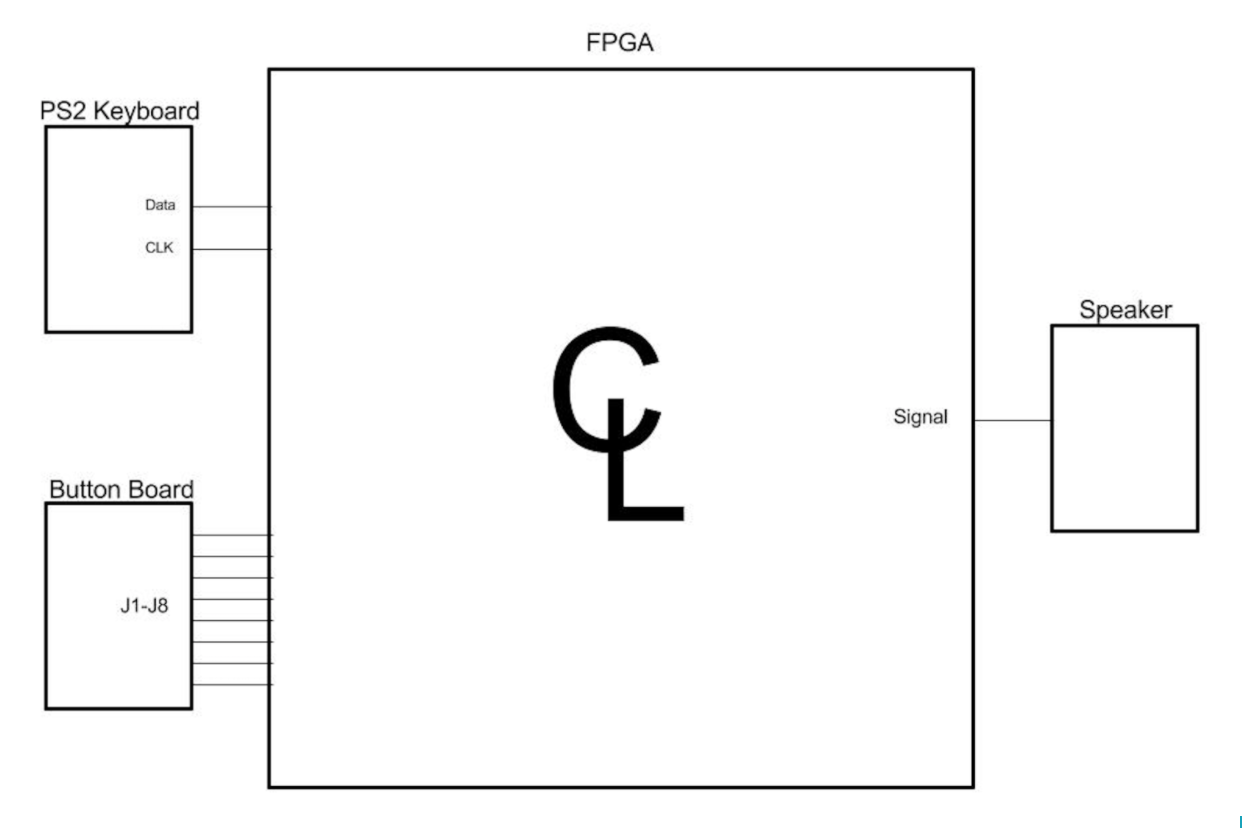
\includegraphics[width=6 in]{./Images/jackPictures/highLevel.png}


Inputs: This reads signals from either a PS${_2}$ keyboard or an 8-button push button board, the one provided in the lab portion of this class. \newline\newline\newline
Outputs: This design outputs a sine wave signal to a speaker which will play one of the eight preset frequencies, the signal of which is selected by the inputs. 
\newline\newline
Description: As shown in the diagram above, the signals are taken from either of the two input options and then sent to the FPGA. In the case of the PS2 keyboard, a data line connects the keyboard to the FPGA using one of the input pins on the FPGA. This data line provides a flow of binary inputs that are read into the logic on the FPGA. In the case of the button board, the buttons J1-J8 are connected to 8 of the input pins on the FPGA, when pressed they will send a logic low reading to the FPGA, if they are not pressed they will send a logic high. When a button is pressed, the FPGA will choose which frequency is played based on the origin of the logic low reading. The speaker has one connection with the FPGA which with send a sine wave through one of the output pins on the FPGA. 


\section{Input Boards}

\subsection{PS2 Keyboard}

\begin{figure}[h]
    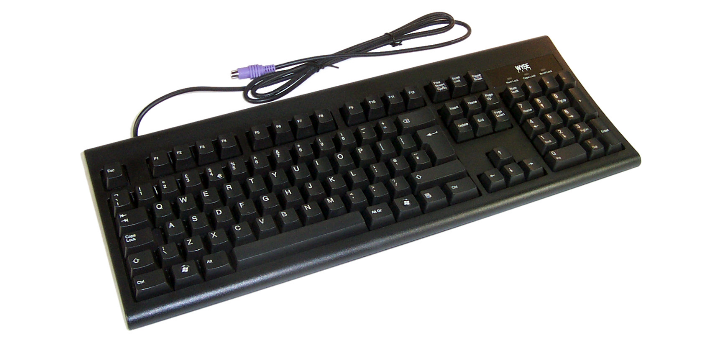
\includegraphics[width=6 in]{Images/ps2keyboard.png}
    \caption{PS${_2}$ Keyboard}
    \label{fig:2}
\end{figure} {floats}

The first input that our design takes in is a PS2 keyboard (pictured above). The keyboard has one wire that connects to board itself to the logic. This wire is a data wire that sends data bit by bit to the logic. This type of communication protocol is known as parallel communication. Since the data is sent bit by bit, a shift register is required to pick up all the bits that are sent. This shift register then sends the N-bits of data when the register is full, then wipes the registers clear and starts reading bits in again. The shift register in our design is 11-bits because 11 bits of data represents a pressed key. Three of those eleven bits are erranous and don’t have a particular use in our design. The middle eight bits hold the information for which key was pressed. However, the data does not start flowing instantly upon connection. A clock value has to be started in order for the data wire to start sending signals. The same clock value is used in the register to update the inputted data. \pagebreak

\subsection{Button Board}

\begin{figure}[h]
    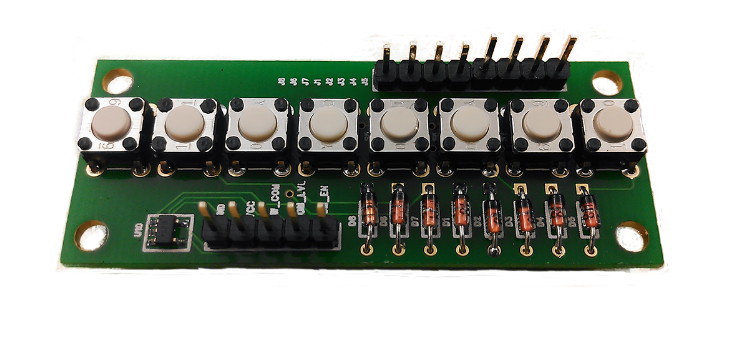
\includegraphics[width=6 in]{./Images/bBoard.png}
    \caption{buttonBoard}
    \label{fig:3}
\end{figure}

The second input that our design is capable of reading is the 8-button push-button board. The picture above is the same model as the device used in the lab portion of this class. This is a very simple implementation of parallel communication protocol which can send 8 bits of information at a time. The controller is used in this design to switch between the 8 pre-set frequency values. There is also a command from the button board to pause and play the currently selected frequency through the speaker.

\section{Modules}

\subsection{Top Module}

    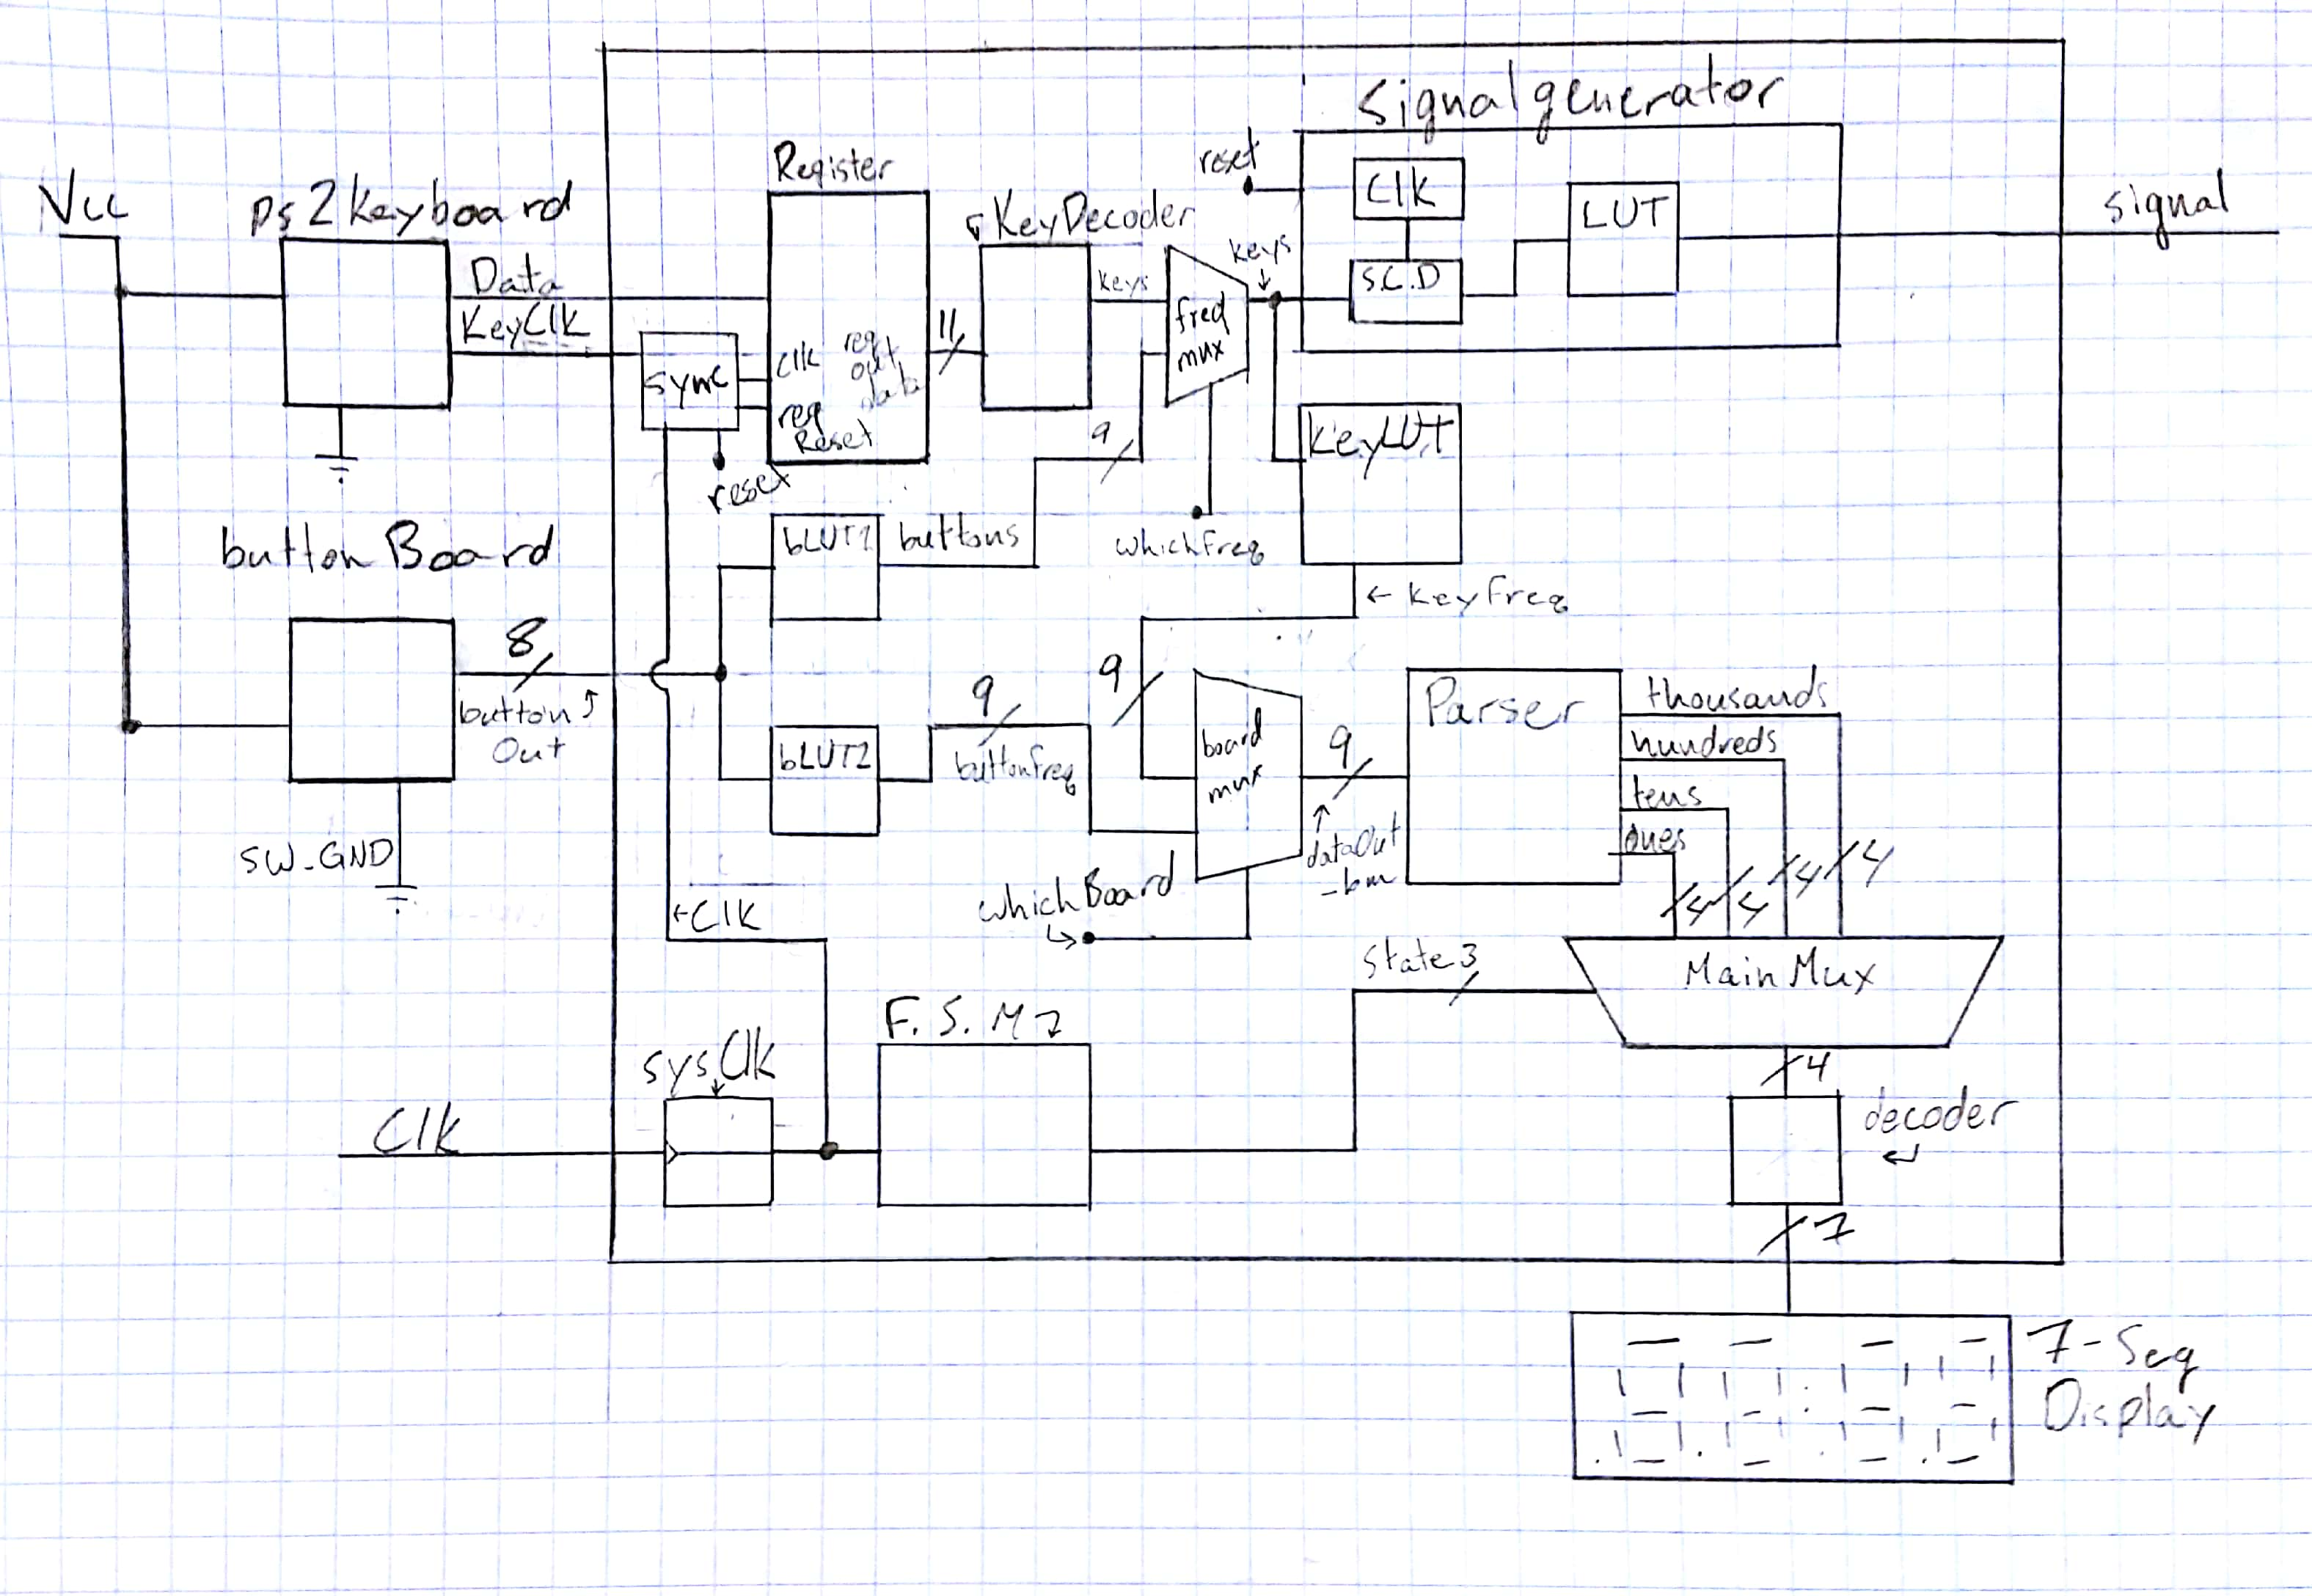
\includegraphics[width=5.5 in]{Images/topLevelSchematic.jpg}


Inputs: This module intakes a 4-bit number representing the decimal value of the current digit being displayed.
\newline\newline
Outputs: This module outputs a 7-bit code that is sent to the 7-segment display that controls which of the segments on the display are illuminated.
\newline\newline
Description: The module is built from a case statement that looks at what the input value represents in decimal form then decides which code to send to the 7-segment display to turn on the right segments to display the decimal number.


\subsection{Register}

    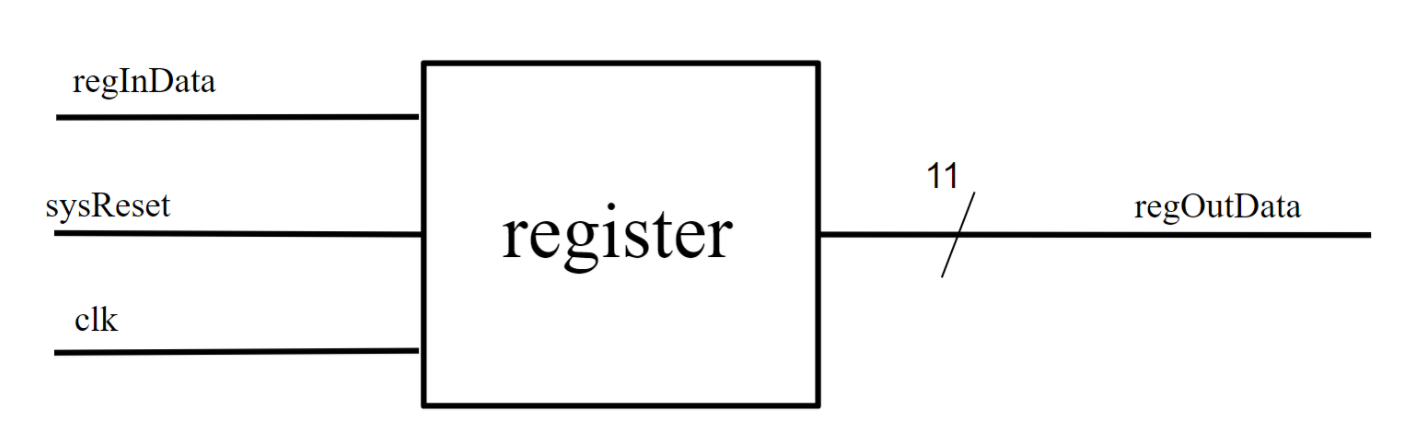
\includegraphics[width=6 in]{./Images/DiagramsYang/register.png}


Inputs: \newline
	regInData from the PS2 keyboard;\newline
    Clk generated from the PS2 keyboard;\newline
    A reset input from clock sync module.\newline\newline
Outputs: 11-bit data line.
\newline\newline
Description: The register takes the keyboard input regInData which comes 1 byte at a time; the register also takes a clk input from the keyboard. It stores 1 byte each time at the rising clock edge; after 11 ticks the 11-bit data line is output as regOutData. It also has a reset input so it can reset the values if the input data is invalid.  


\subsection{Keyboard Decoder}

    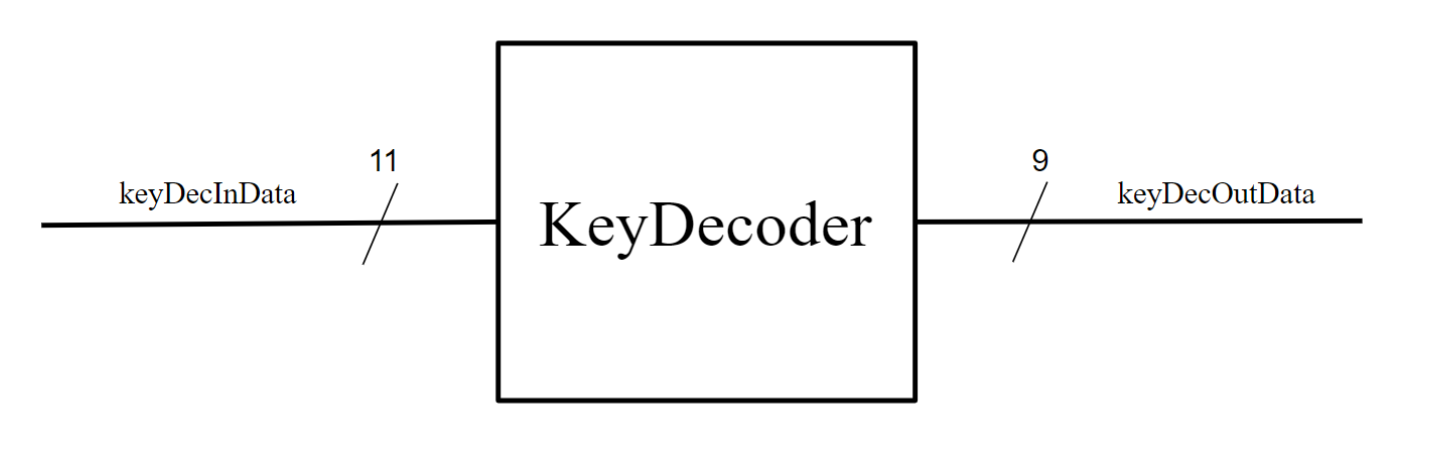
\includegraphics[width=6in]{./Images/DiagramsYang/keyDec.png}


Inputs: This module intakes a 4-bit number representing the decimal value of the current digit being displayed.
\newline\newline
Outputs: This module outputs a 7-bit code that is sent to the 7-segment display that controls which of the segments on the display are illuminated.
\newline\newline
Description: The module is built from a case statement that looks at what the input value represents in decimal form then decides which code to send to the 7-segment display to turn on the right segments to display the decimal number.


\subsection{Key Look Up Table}

    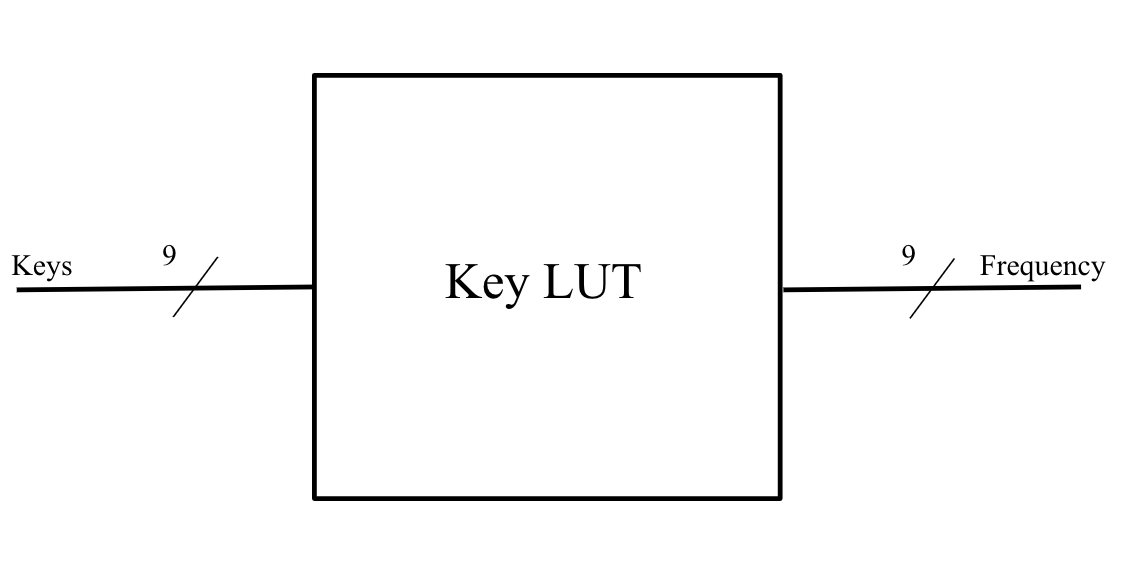
\includegraphics[width=6 in]{./Images/jackPictures/keyLUT.png}


Inputs: This module inputs a 9-bit frequency key that is related to an actual frequency value.
\newline\newline
Outputs: This module outputs a 9-bit number that represents the decimal value for the selected frequency.
\newline\newline
Description: The module is constructed from a case statement that selects which frequency value to send out based on what frequency key was inputted. If the frequency key was inputted for the first frequency, then the output of the module would be the binary representation of the decimal value for the first frequency.


\subsection{Button Look Up Table 1}

    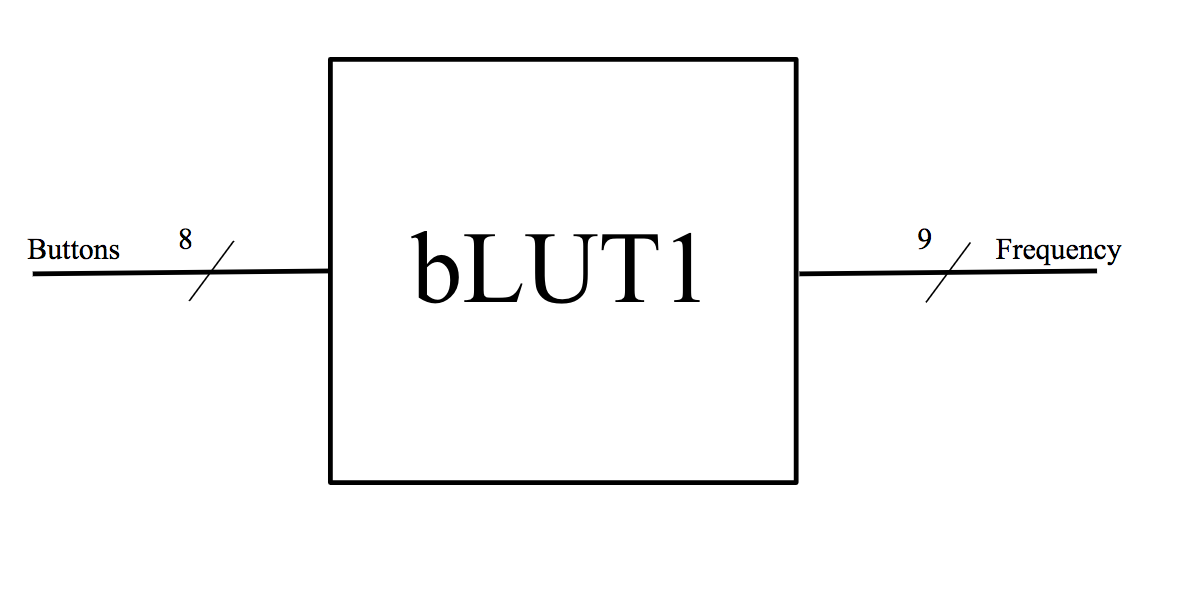
\includegraphics[width=6 in]{./Images/jackPictures/blut1.png}


Inputs: This module intakes 8-bits of data from the button board.
\newline\newline
Outputs: This module outputs a 9-bit frequency key value
\newline\newline
Description: The module is built from a case statement that looks at the buttons pressed, and then sends a key value to the signal generator which lets the signal generator which frequency to output.


\subsection{Button Look Up Table 2}

    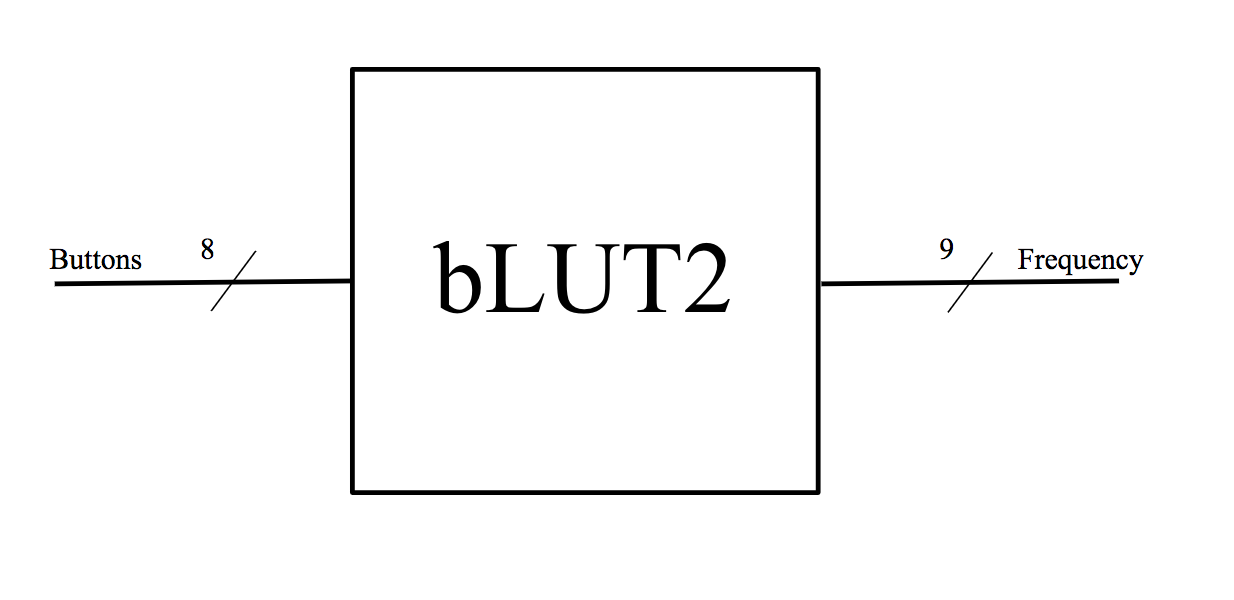
\includegraphics[width=6 in]{./Images/jackPictures/blut2.png}


Inputs: This module intakes 8-bits of data from the button board.
\newline\newline
Outputs: This module outputs a 9-bit value that represents the decimal value of the frequency selected.
\newline\newline
Description: The module is built from a case statement that looks at what buttons are pressed, then decides which decimal frequency value corresponds with the button pressed, then sends the frequency value in binary form so it can be displayed by the 7-segment display decoder.


\subsection{Frequency Mux}

    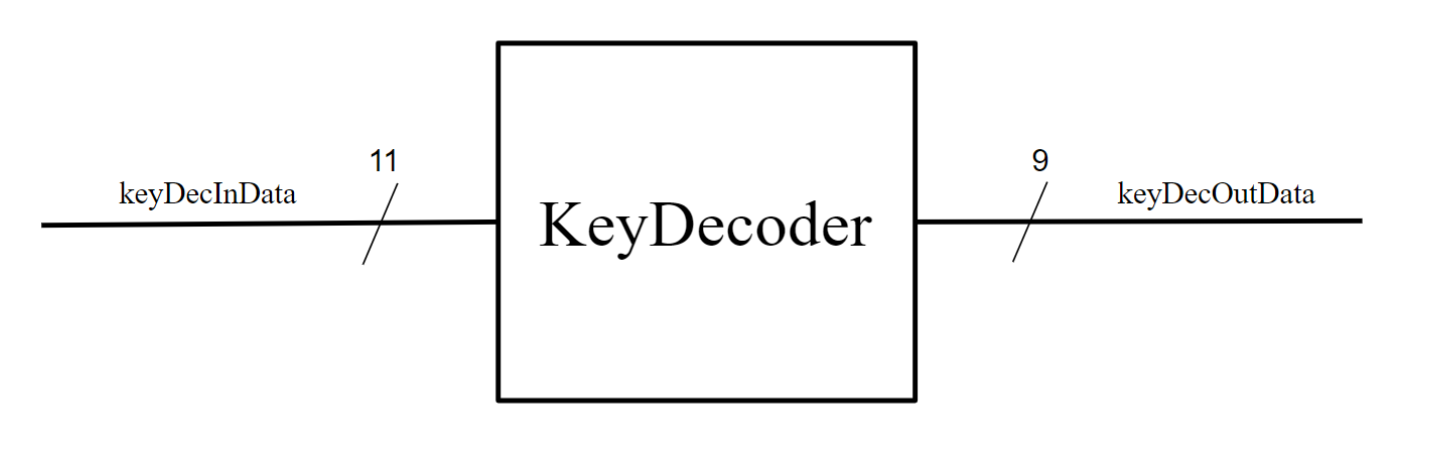
\includegraphics[width=6 in]{./Images/DiagramsYang/keyDec.png}


Inputs: keyFreqIn from the KeyDecoder module and bbFreqIn from the bLUT1 module;
\newline\newline
Outputs: dataOut${_fm}$;
\newline\newline
Description: This multiplexer takes the output from the KeyDecoder (keyDecOutData) and the output from bLUT1 module (buttons), which are both binary values; then it selects one between the two to pass straight through the output  (dataOut${_fm}$). When the 1-bit input whichFreqOut is ‘0’, the keyboard data is being passed; and when it is ‘1’, the button board data is being passed. The output goes to keyLUT which determines the binary value of the frequency being displayed on the seven segment. 


\subsection{Board Mux}


    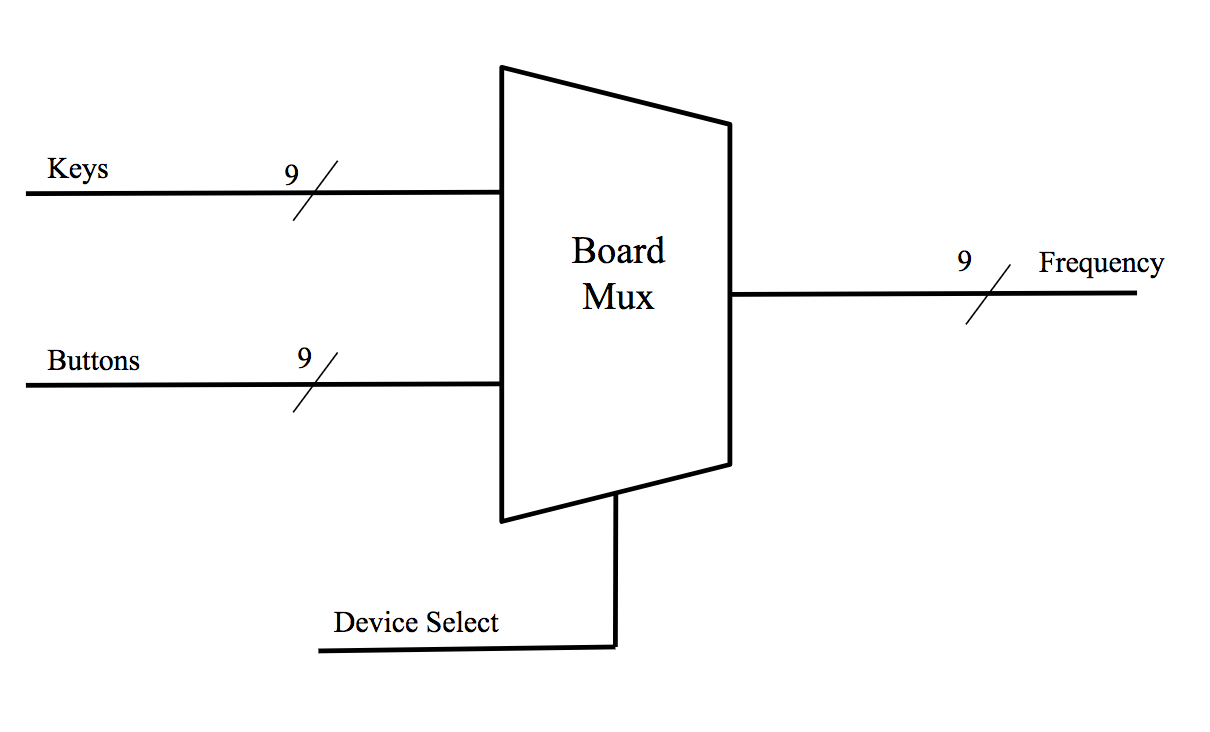
\includegraphics[width=6 in]{./Images/jackPictures/boardMUX.png}

Inputs: This module intakes 9 bits representing a decimal frequency value from both the keyboard and the button board. It also intakes a select value.
\newline\newline
Outputs: This module outputs 9 bits representing a decimal frequency value.
\newline\newline
Description: The module is built from a case statement that determines which frequency value gets sent to the 7-segment display decoder, based on what the input type is active.


\subsection{Signal Generator Top Level}

\begin{figure}[h]
    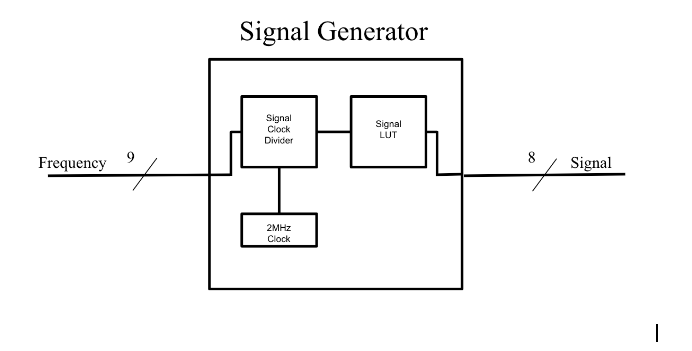
\includegraphics[width=6 in]{./Images/chasePictures/sigTopMod.png}
    \caption{sigGenTopLevel}
    \label{fig:12}
\end{figure}

The signal generator is told which key is pressed by the decoder. It then outputs an 8 bit binary number to the DAC representing the height of the sound wave at each successive moment in time. A new 8 bit value is sent to the DAC a few hundred thousand times per second.


\subsection{Signal Clock Divider}

\begin{figure}[h]
    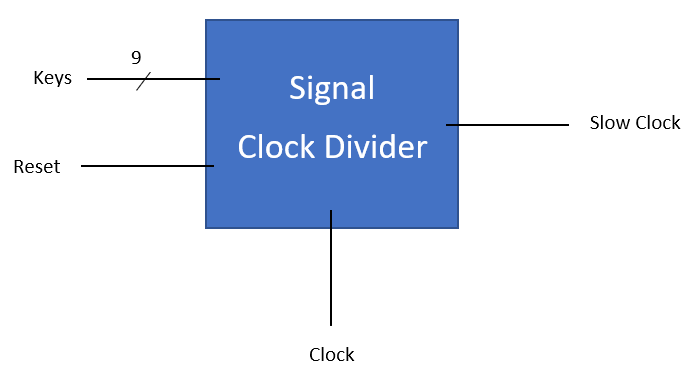
\includegraphics[width=6 in]{./Images/chasePictures/SignalClockDivider.PNG}
    \caption{Signal Clock Divider}
    \label{fig:13}
\end{figure}

The signal clock divider sub-module takes the built-in 2.08 Mhz clock signal and slows it down by an amount dependent on which frequency was selected. It accomplishes this by counting a specific number of clock edges from the 2.08 Mhz clock, and flipping its own output clock signal when it reaches that specific number.
\newline\newline
This specific number is determined with a look-up table: each button corresponds with a single entry in the lookup table.


\subsection{Signal Look Up Table}

\begin{figure}[h]
    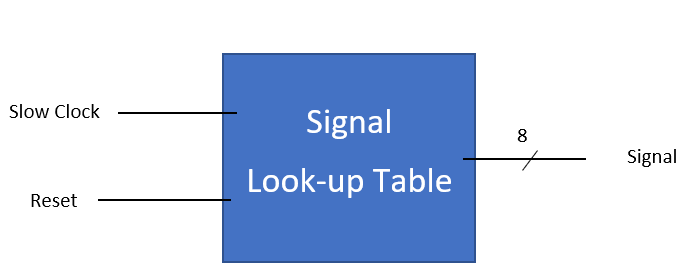
\includegraphics[width=6 in]{./Images/chasePictures/SIgnalLUT.PNG}
    \caption{sigLUT}
    \label{fig:14}
\end{figure}

The signal look-up table submodule takes the slow clock as an input and outputs the 8-bit number representing the height of the sine wave. Filling the entries of the lookup table was one of the hardest parts of the project, because there is no way to directly compute sine using SystemVerilog.
\newline\newline
Our solution was to write a program in C++ to generate the verilog code. The code from that file was then copied and pasted into our program. The C++ code that generated said code is included below.


\subsection{System Clock}

\begin{figure}[h]
    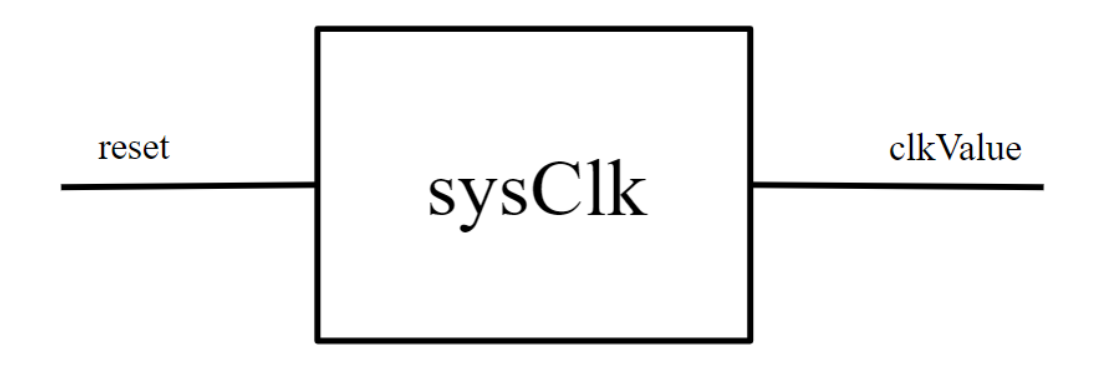
\includegraphics[width=6 in]{./Images/DiagramsYang/sysClk.png}
    \caption{Sync}
    \label{fig:16}
\end{figure}

Inputs: reset;
\newline\newline
Outputs: clkValue;
\newline\newline
Description: This module accesses the FPGA’s chip oscillator and generate the 2.08 MHz system clock output.


\subsection{Free State Machine}

\begin{figure}[h]
    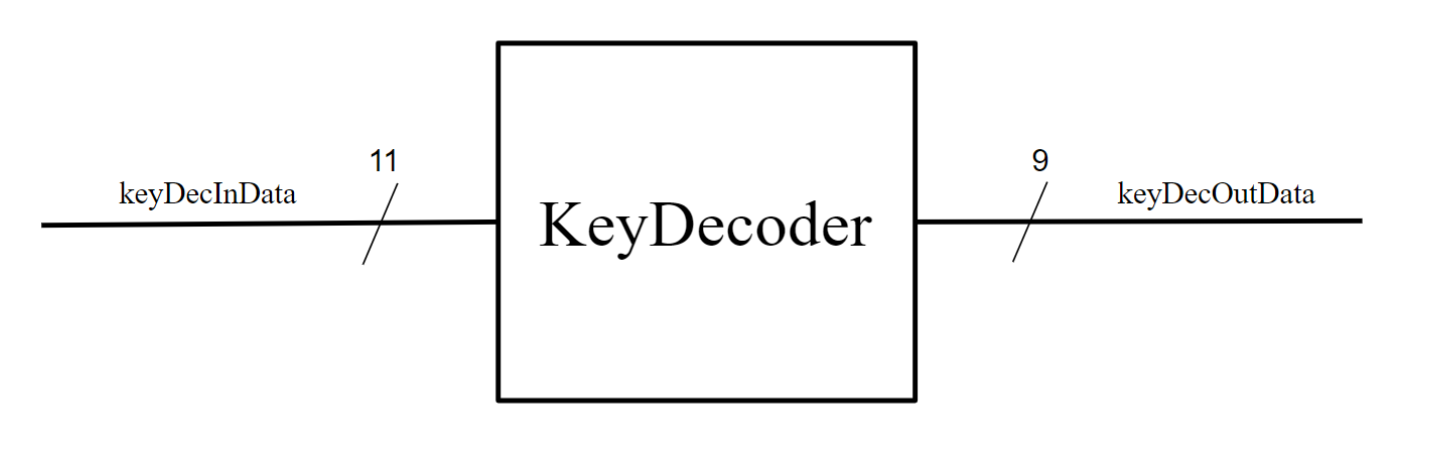
\includegraphics[width=6 in]{./Images/DiagramsYang/keyDec.png}
    \caption{Sync}
    \label{fig:17}
\end{figure}

nputs: This module intakes a clock value, in the design the clock is set to the FPGA’s oscillating frequency of 2.08MHz.
\newline\newline
Outputs: This module outputs a 3-bit state value.
\newline\newline
Description: This module cycles through four different states, one for each digit that can be displayed on the 7-segment display, with the initial state set to the first digit. On the rising edge of the clock value, the state is changed which changes the digit which is illuminated on the display.


\section{Appendix}

\subsection{Code}

\begin{enumerate}

\item Top Module

    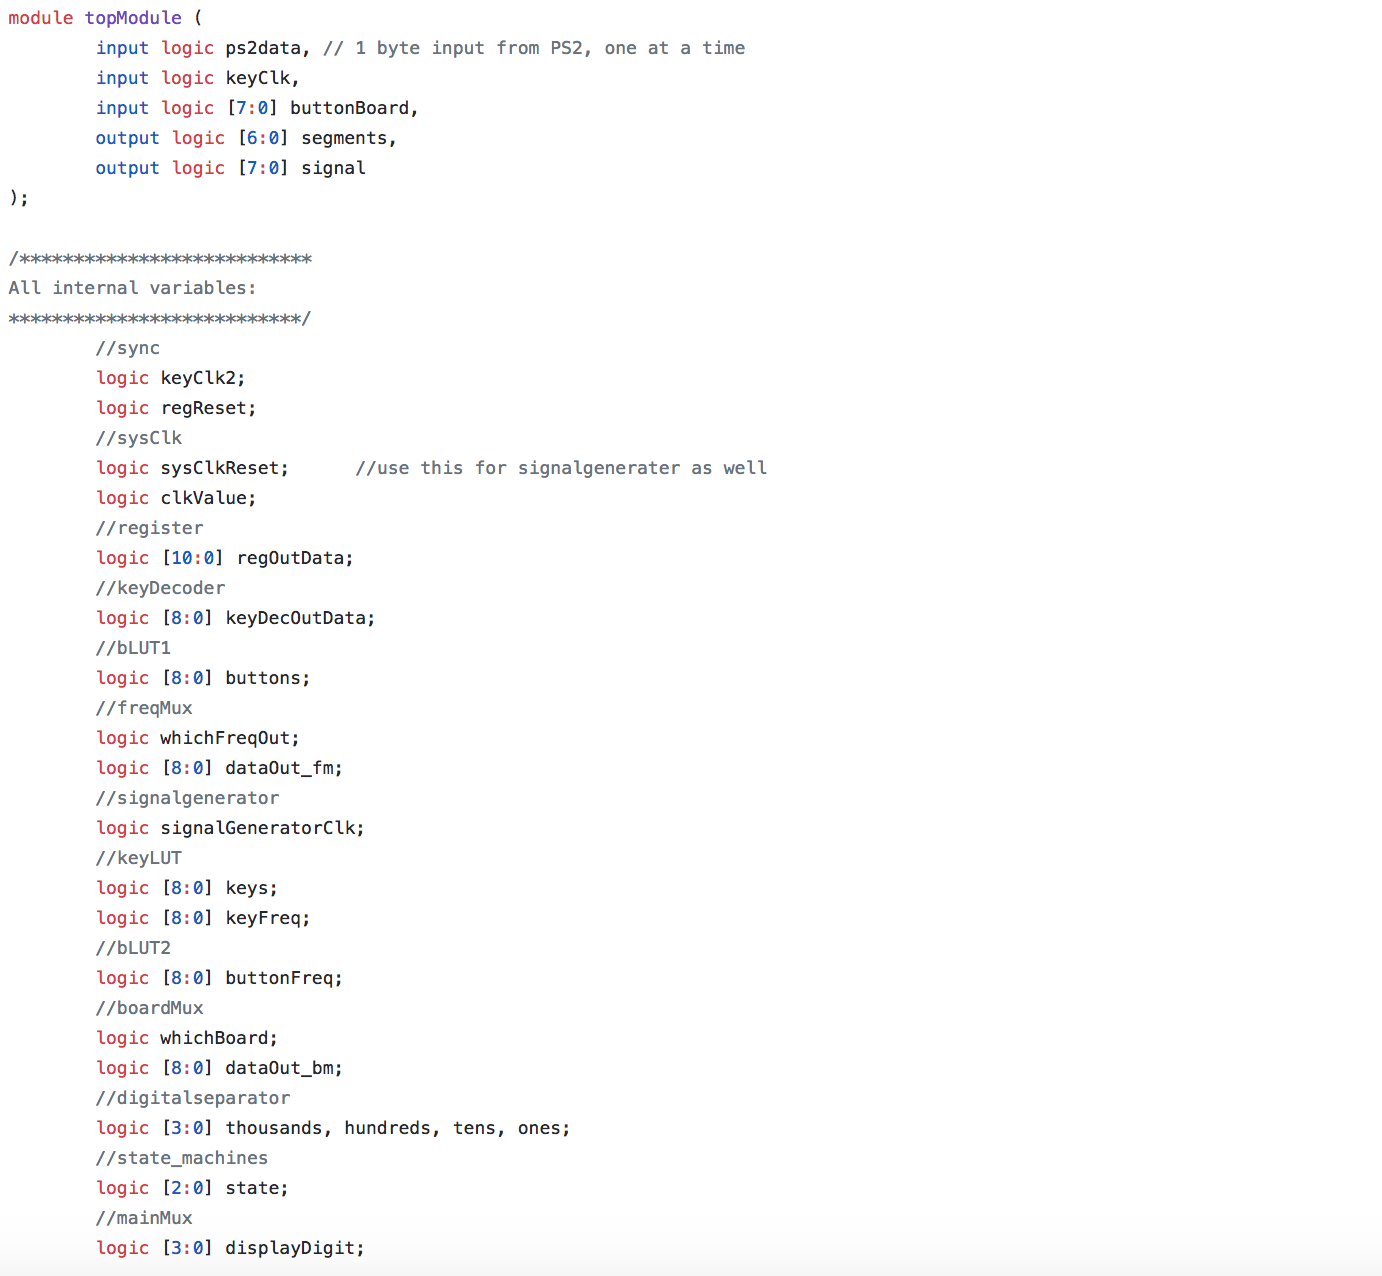
\includegraphics[width=6 in]{./Images/Archive/1-TopMod1.png}

    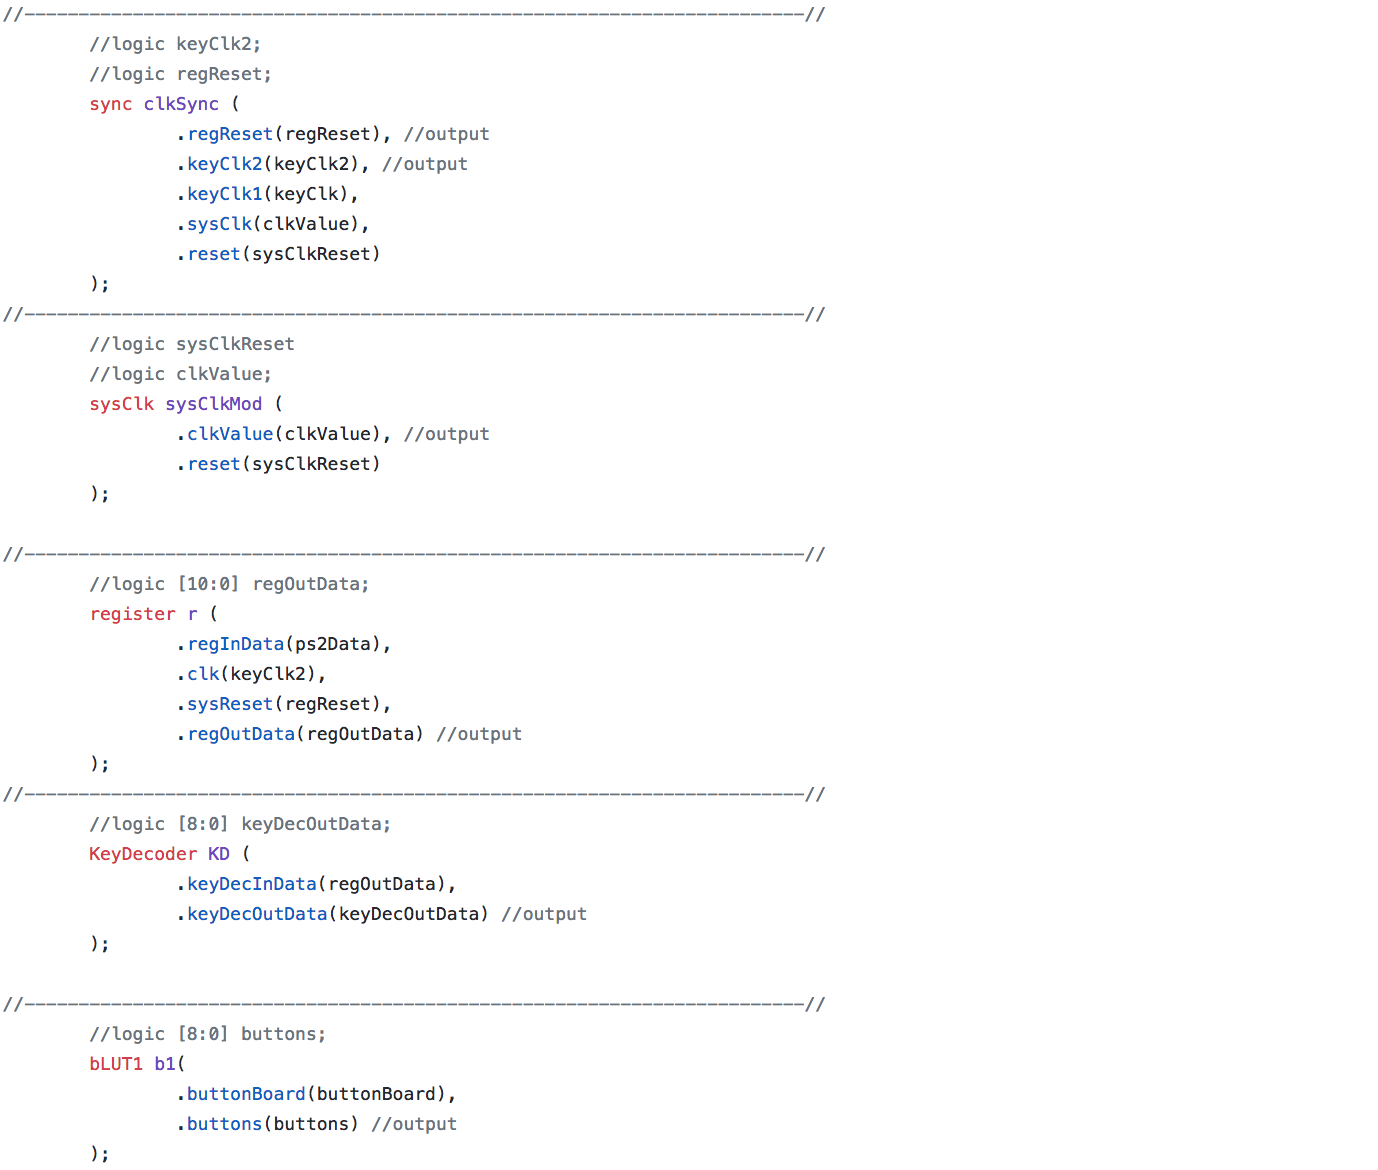
\includegraphics[width=6 in]{./Images/Archive/1-TopMod2.png}

    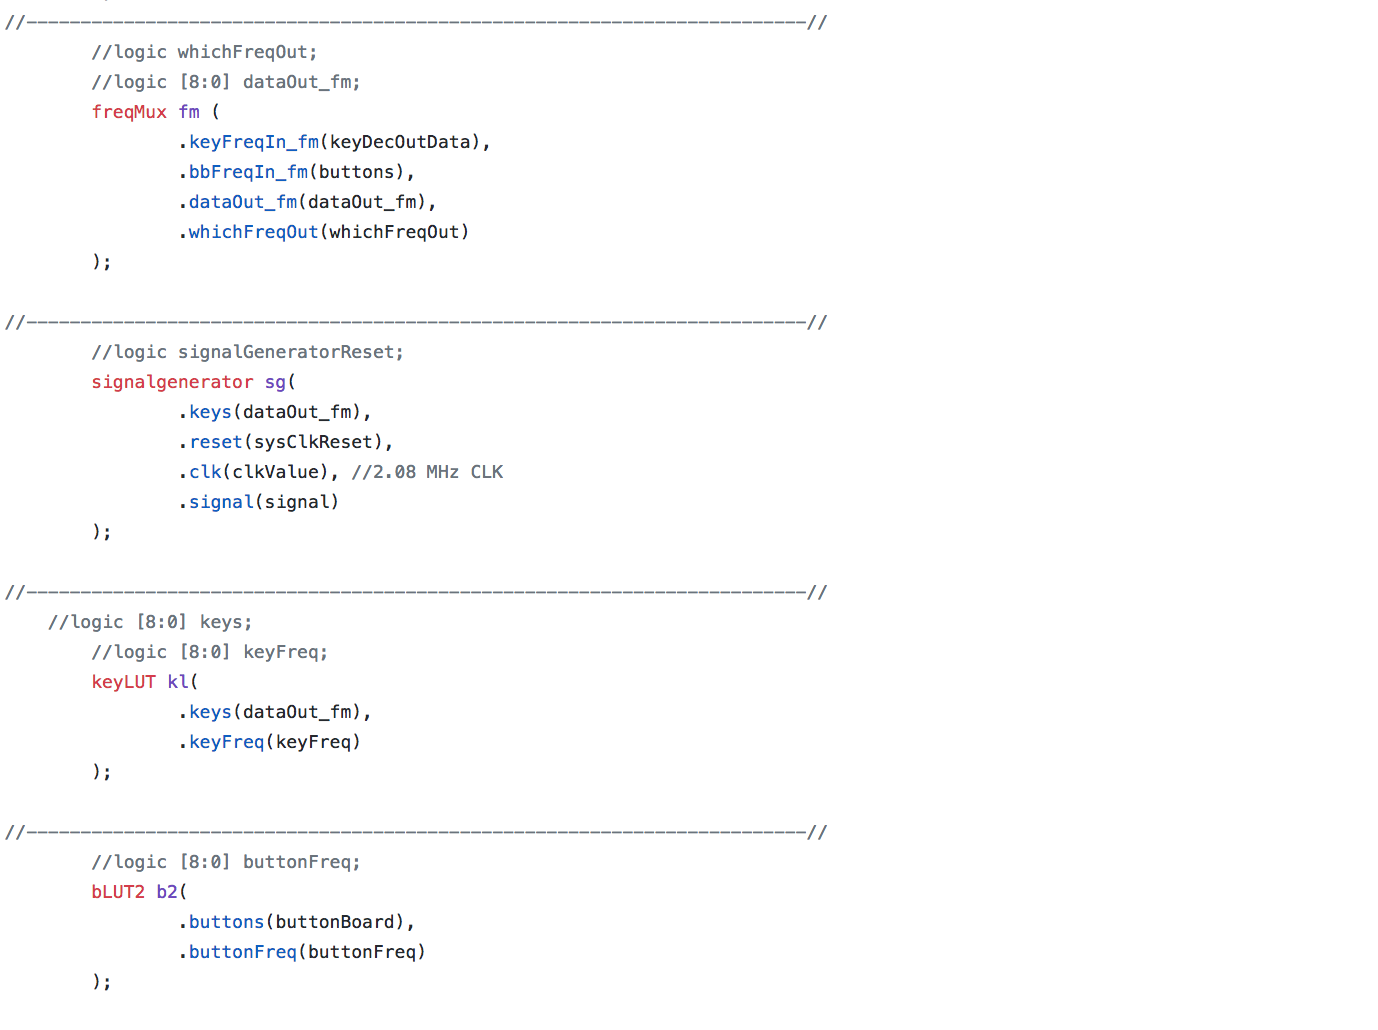
\includegraphics[width=6 in]{./Images/Archive/1-TopMod3.png}

    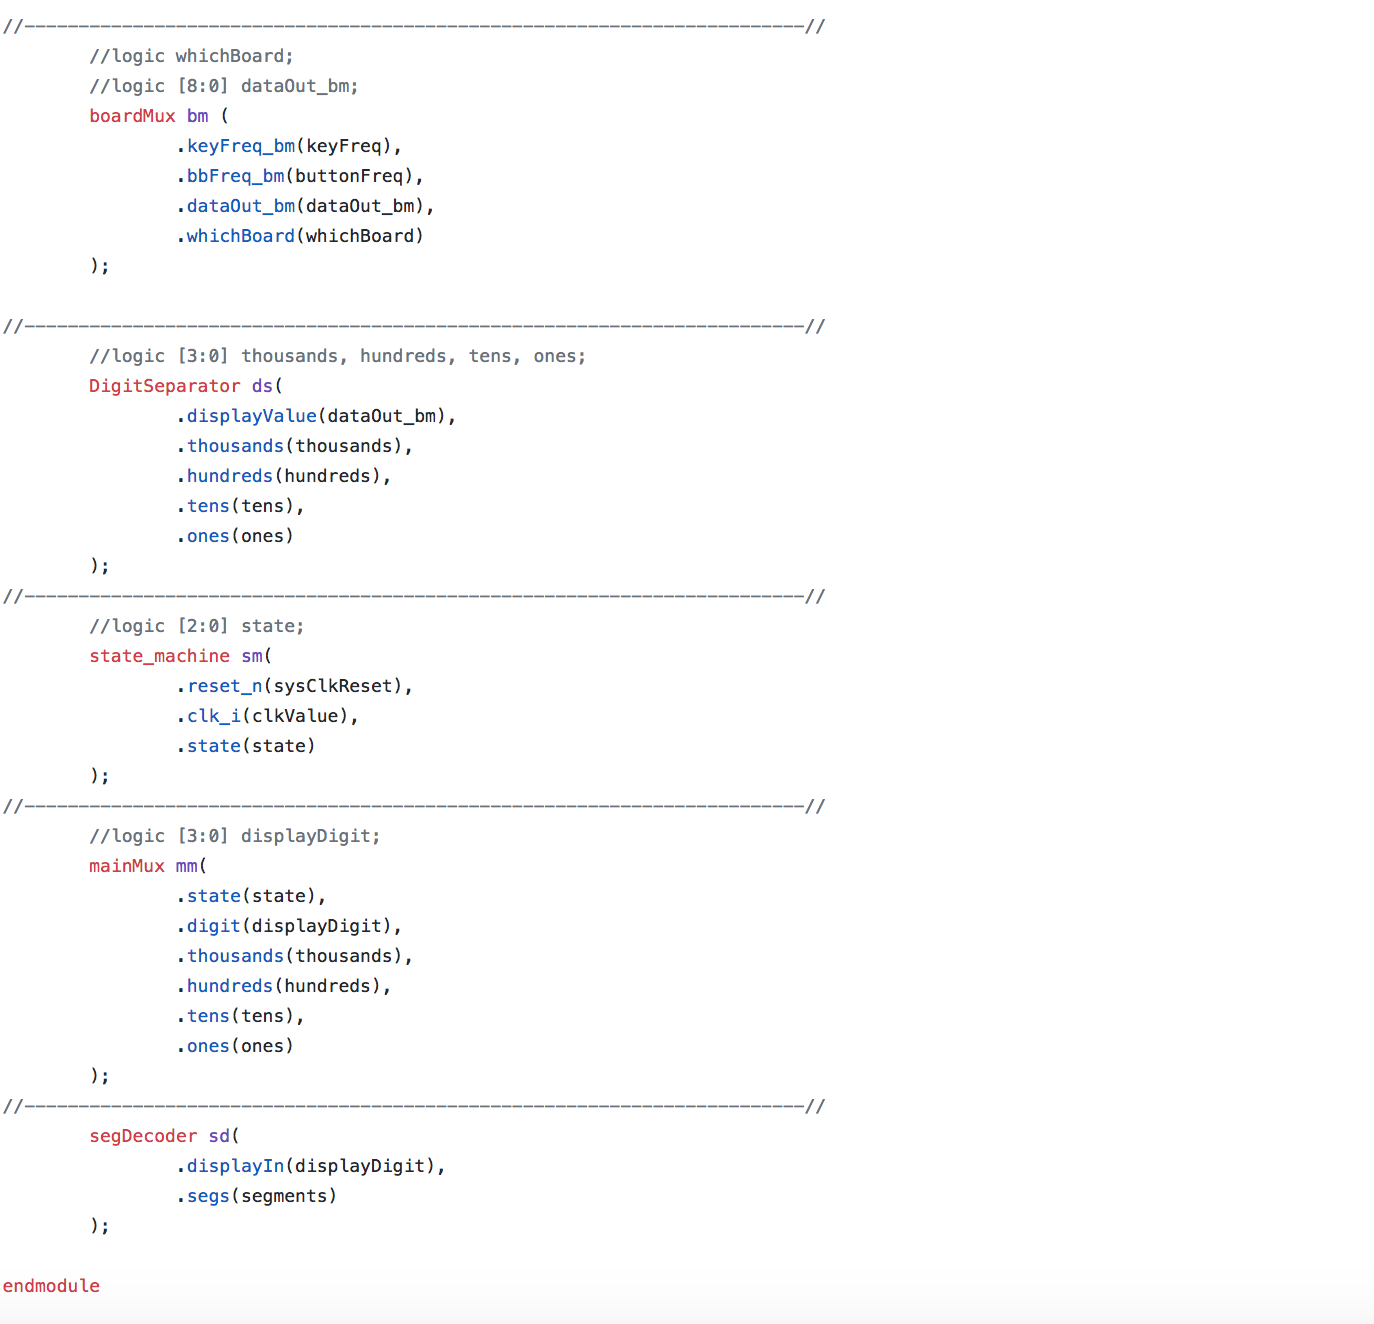
\includegraphics[width=6 in]{./Images/Archive/1-TopMod4.png}


\item Register


    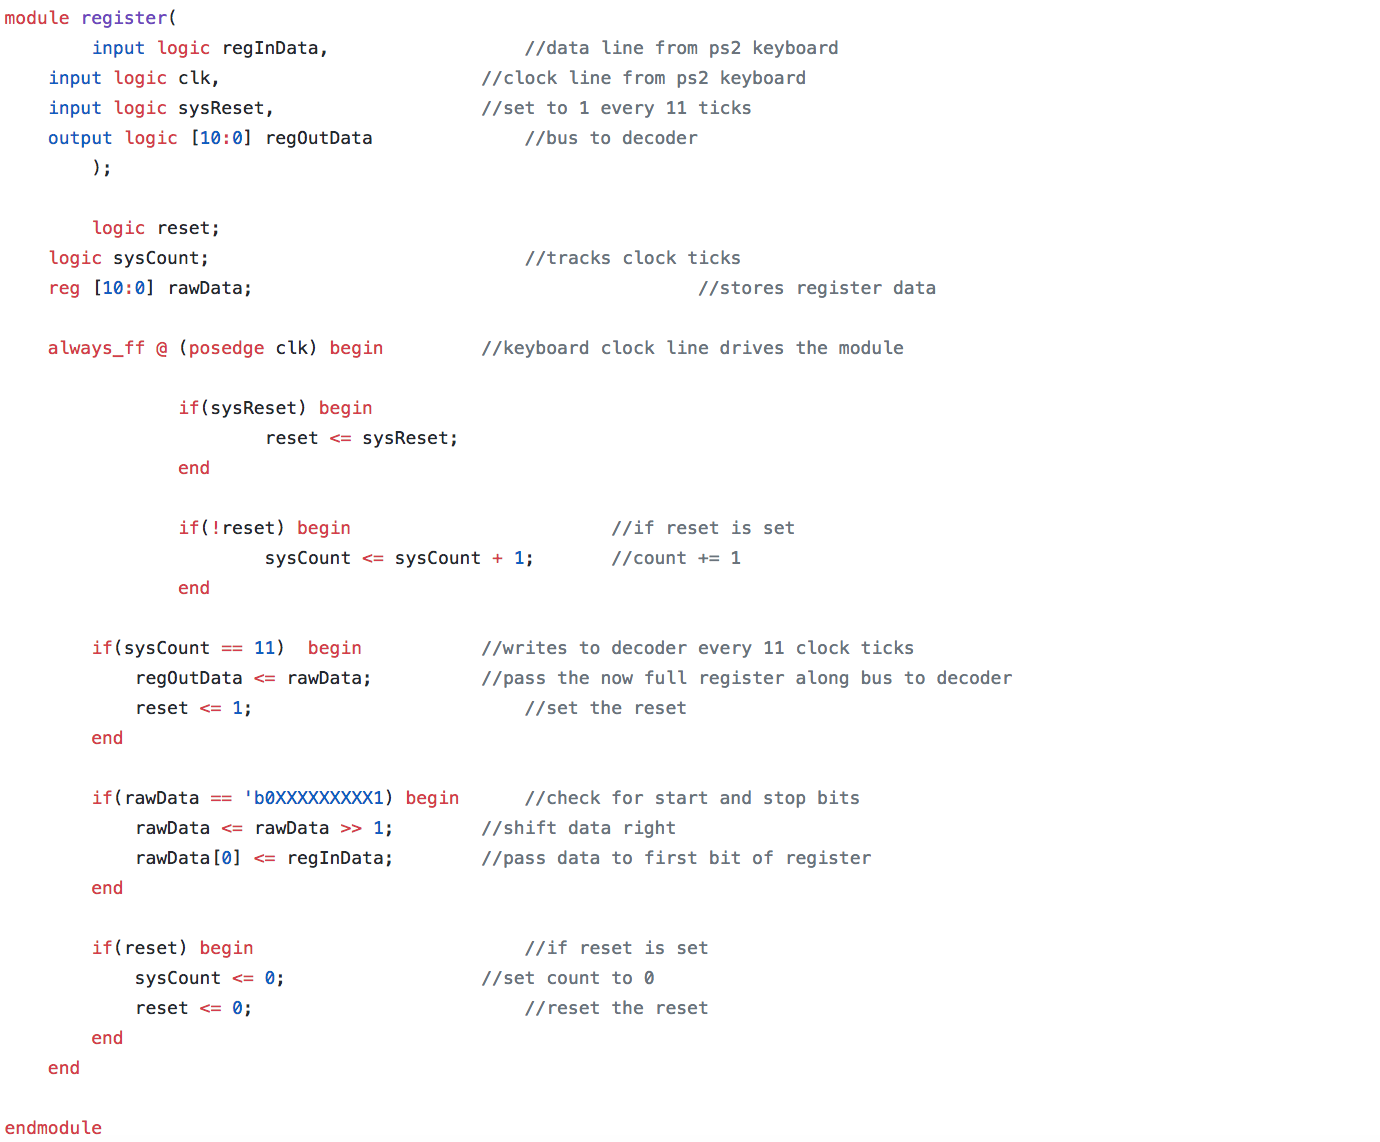
\includegraphics[width=6 in]{./Images/Archive/2-Register.png}


\item Key Decoder


    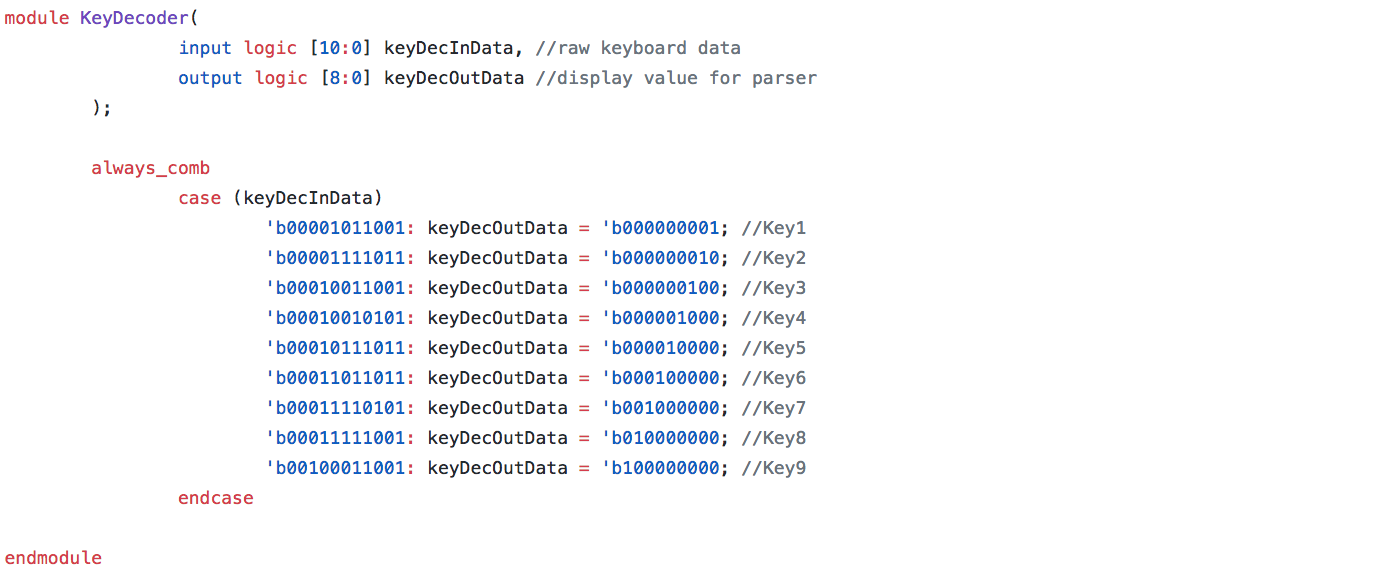
\includegraphics[width=6 in]{./Images/Archive/3-KeyDecoder.png}


\item Key LUT

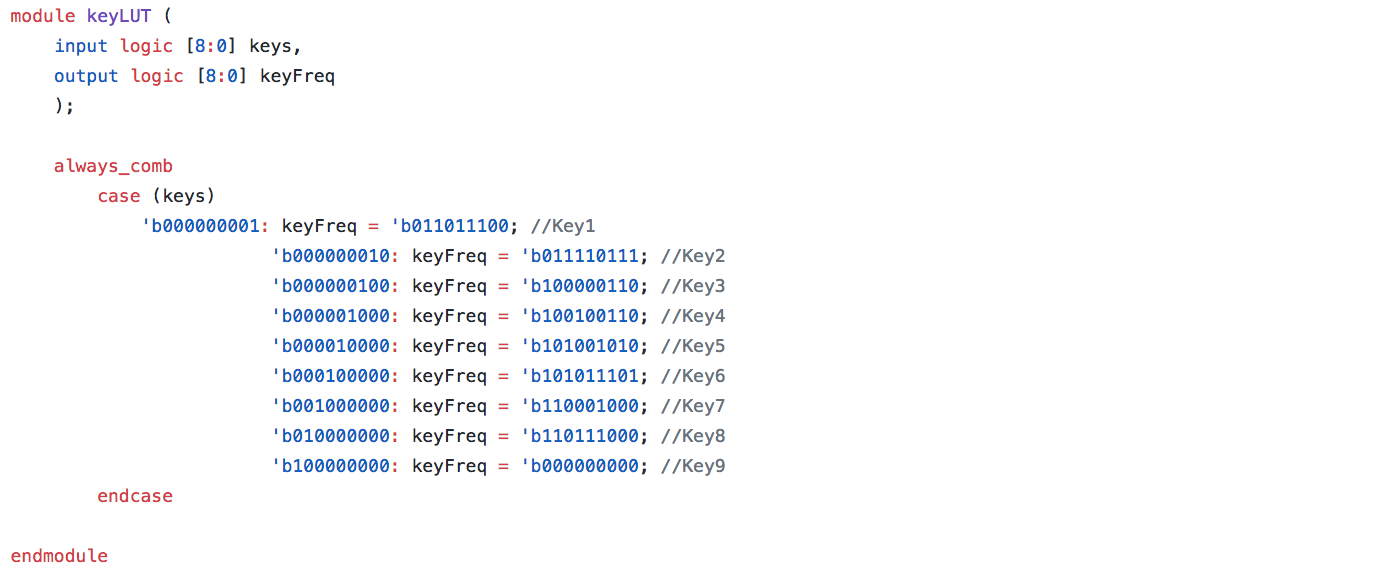
\includegraphics[width=6 in]{./Images/Archive/4-KeyLUT.png}

\item Button LUT 1 

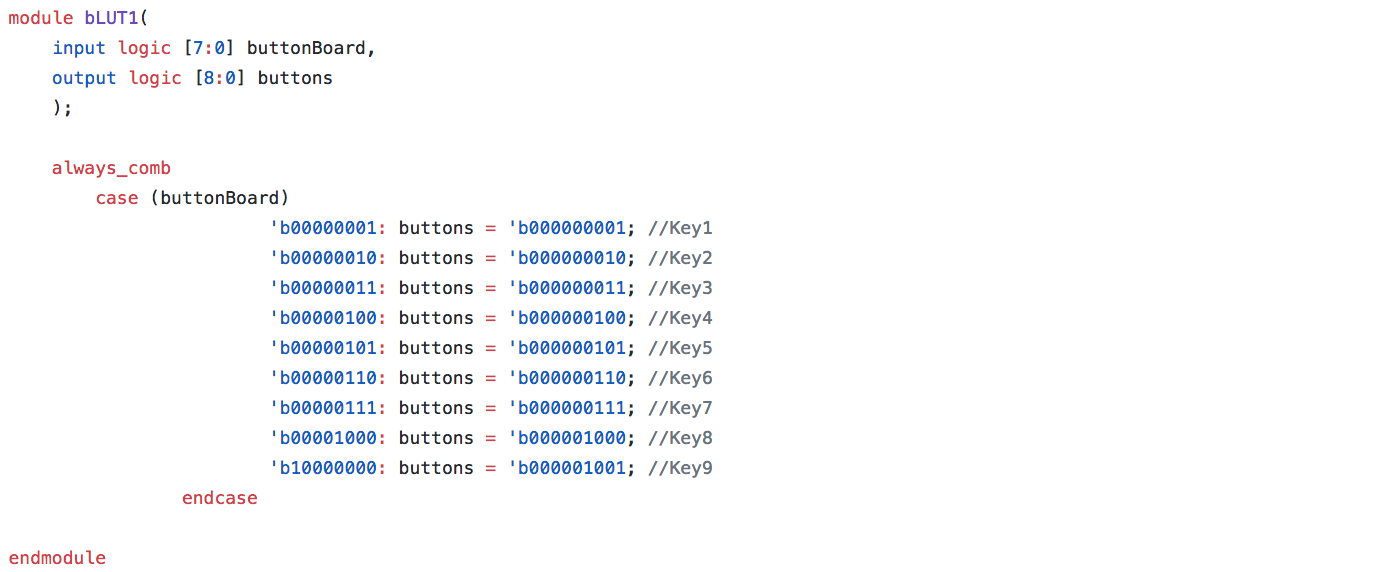
\includegraphics[width=6 in]{./Images/Archive/5-BLUT1.png}

\item Button LUT 2

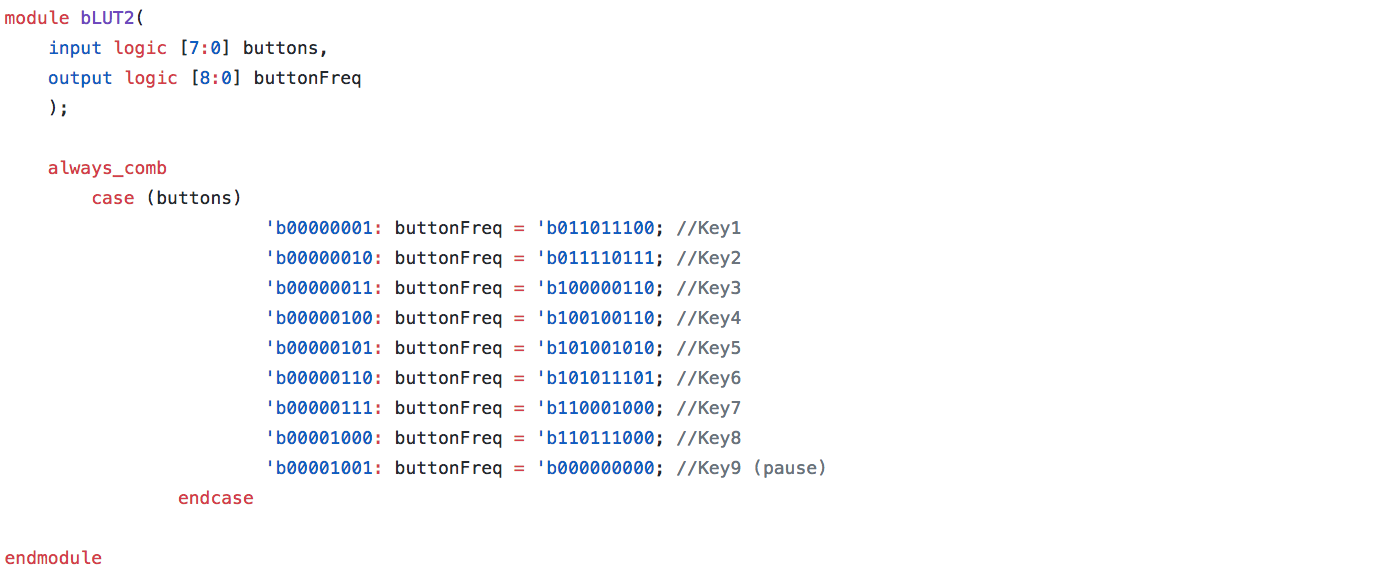
\includegraphics[width=6 in]{./Images/Archive/6-BLUT2.png}

\item Button Frequency Mux

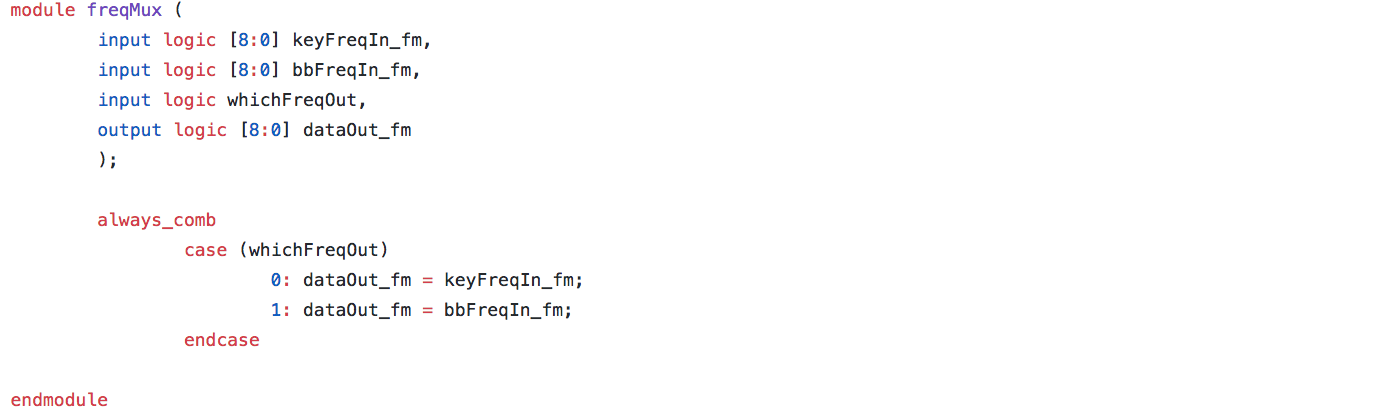
\includegraphics[width=6 in]{./Images/Archive/7-FrequencyMux.png}

\item Board Mux

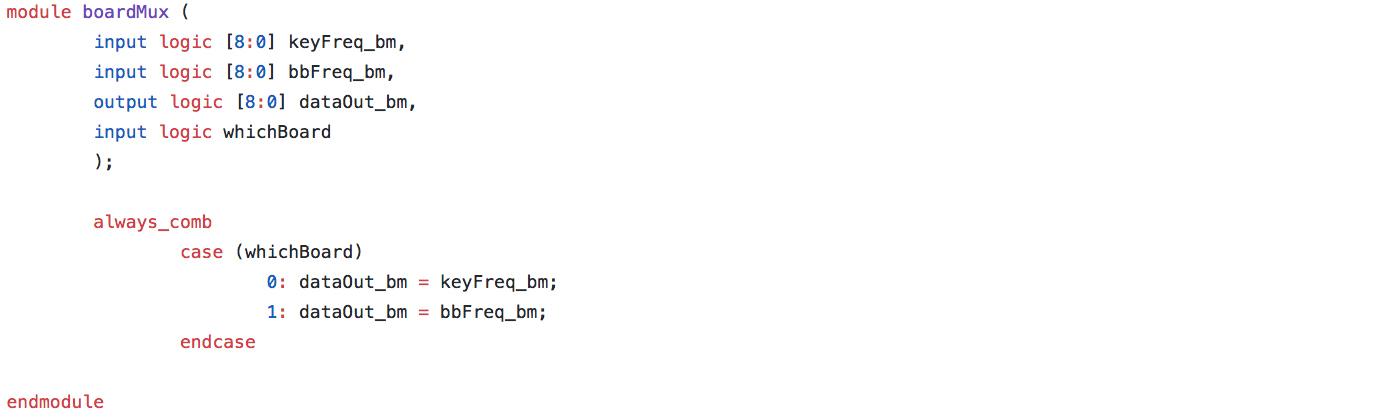
\includegraphics[width=6 in]{./Images/Archive/8-BoardMux.png}

\item Signal Top Level

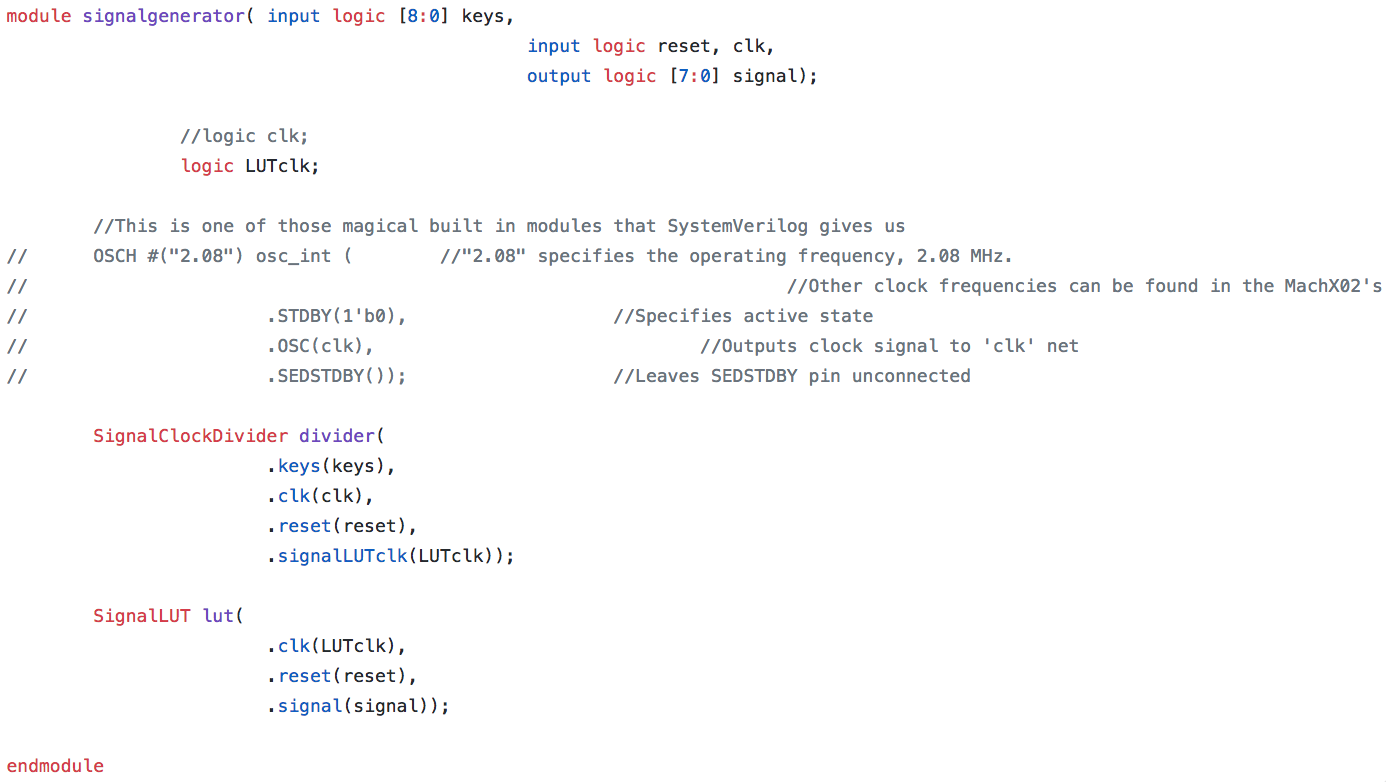
\includegraphics[width=6 in]{./Images/Archive/9-SignalTopLevel.png}

\item Signal Clock Divider

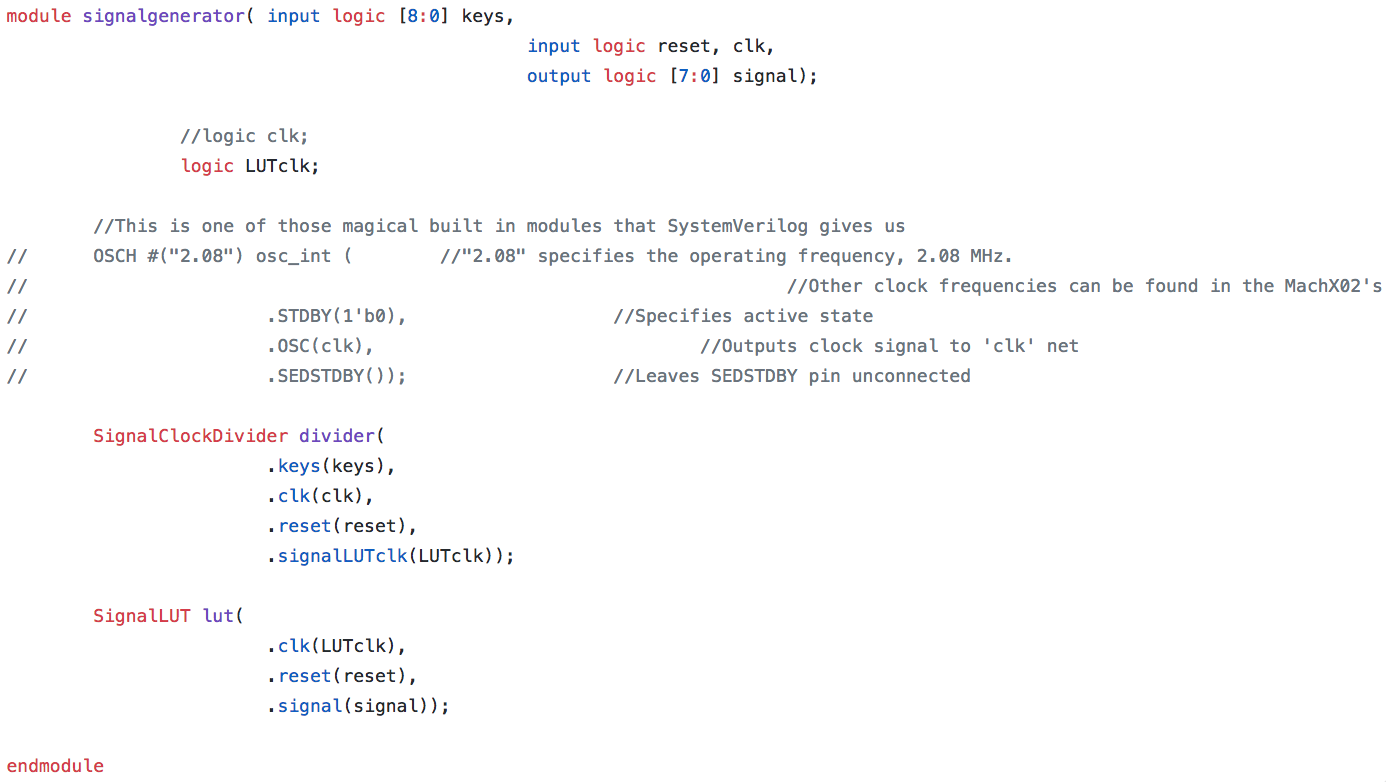
\includegraphics[width=6 in]{./Images/Archive/9-SignalTopLevel.png}


\item Signal LUT

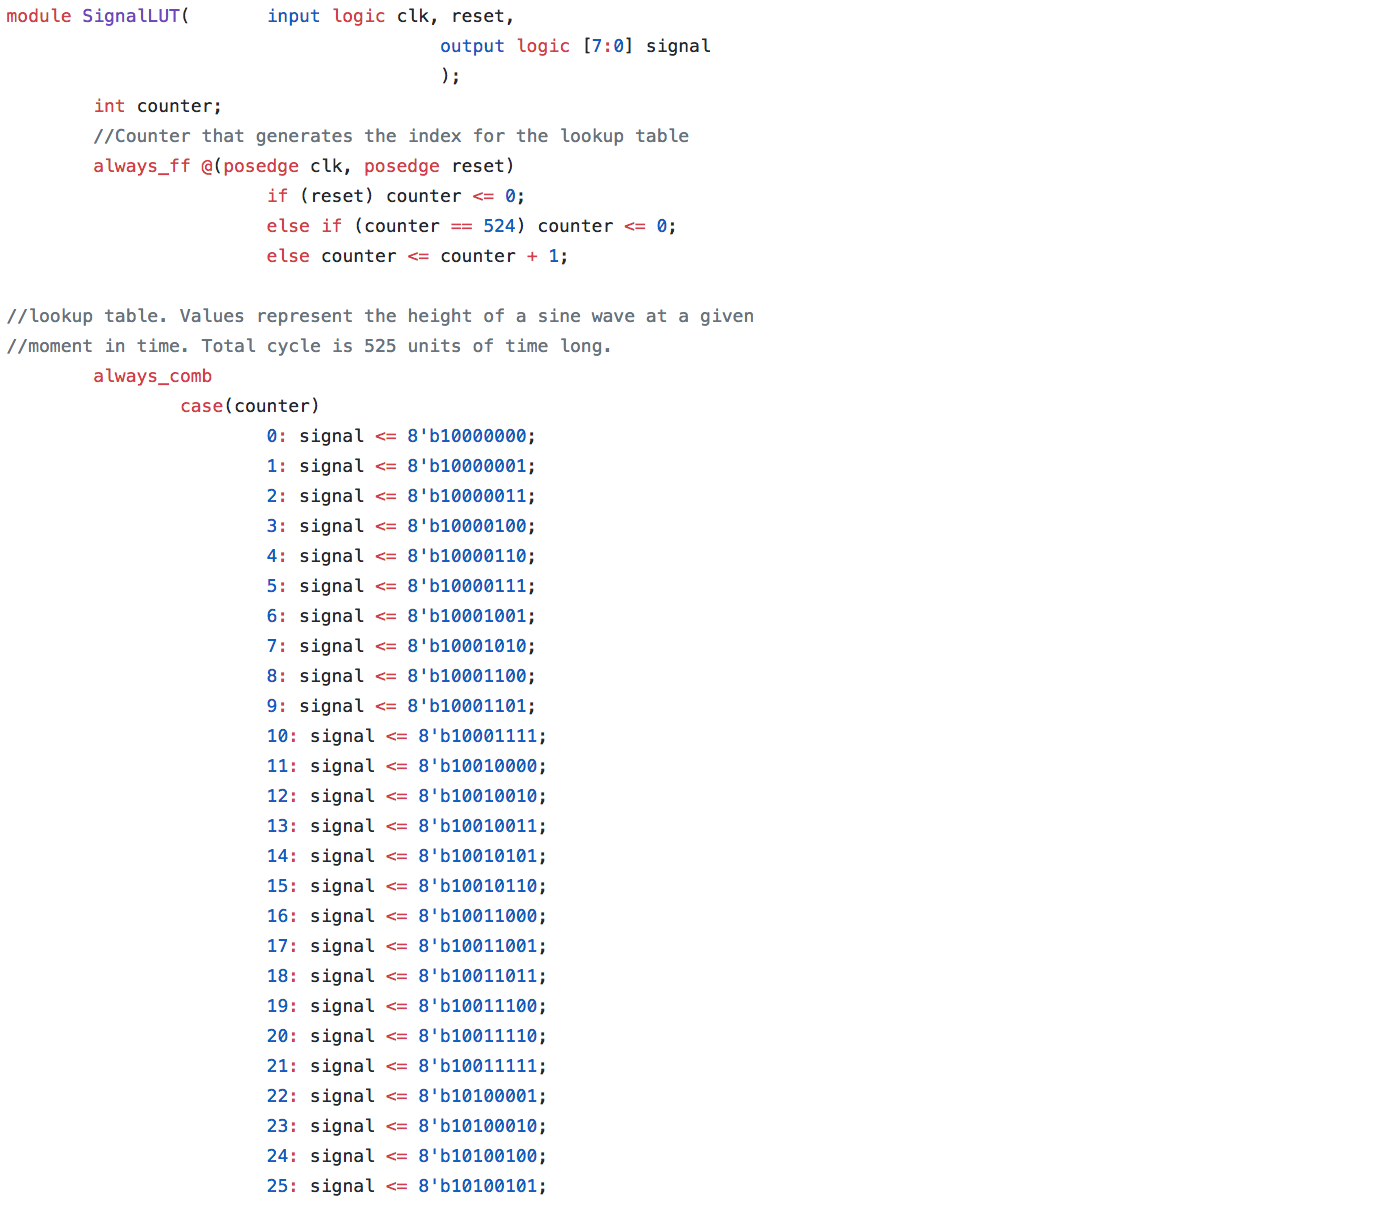
\includegraphics[width=6 in]{./Images/Archive/11-SignalLUT.png}

\item System Clock

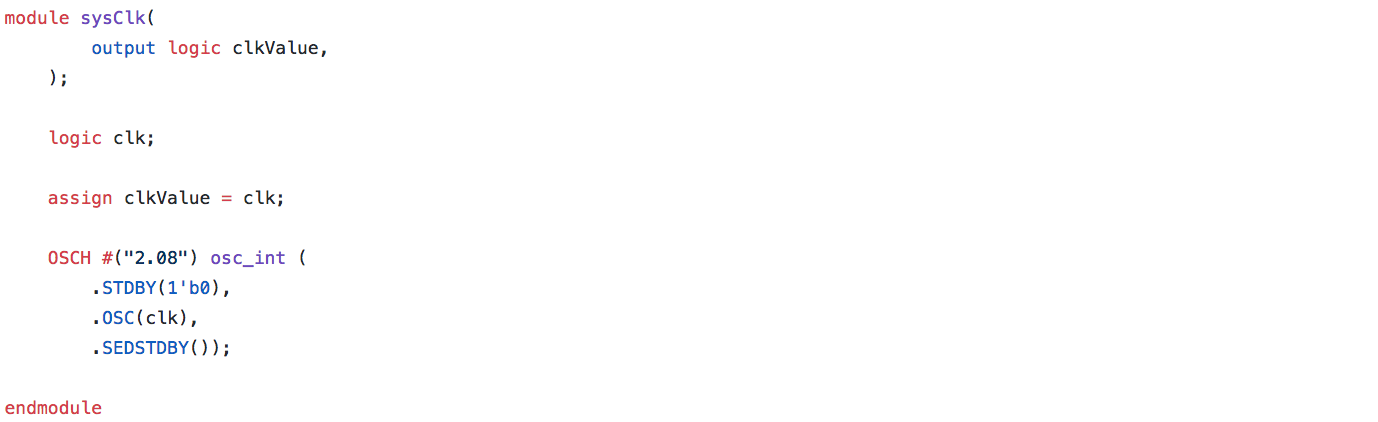
\includegraphics[width=6 in]{./Images/Archive/13-SystemClock.png}

\item State Machine

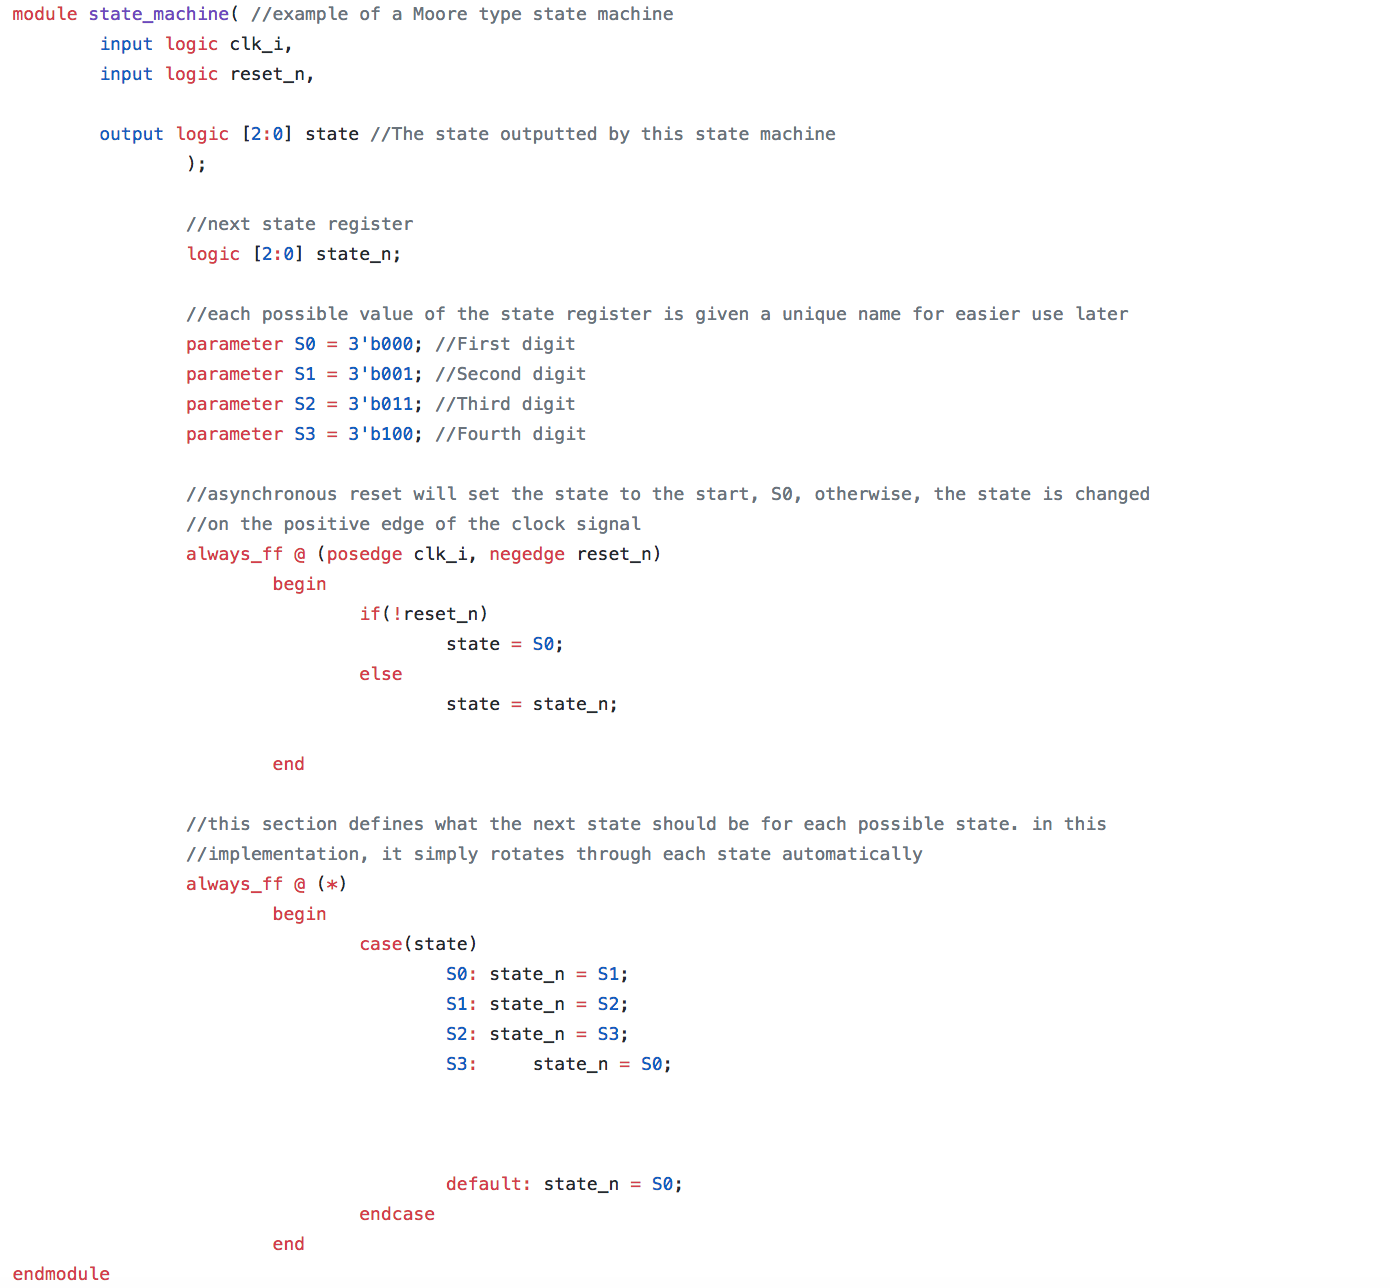
\includegraphics[width=6 in]{./Images/Archive/14-StateMachine.png}

\item Parser

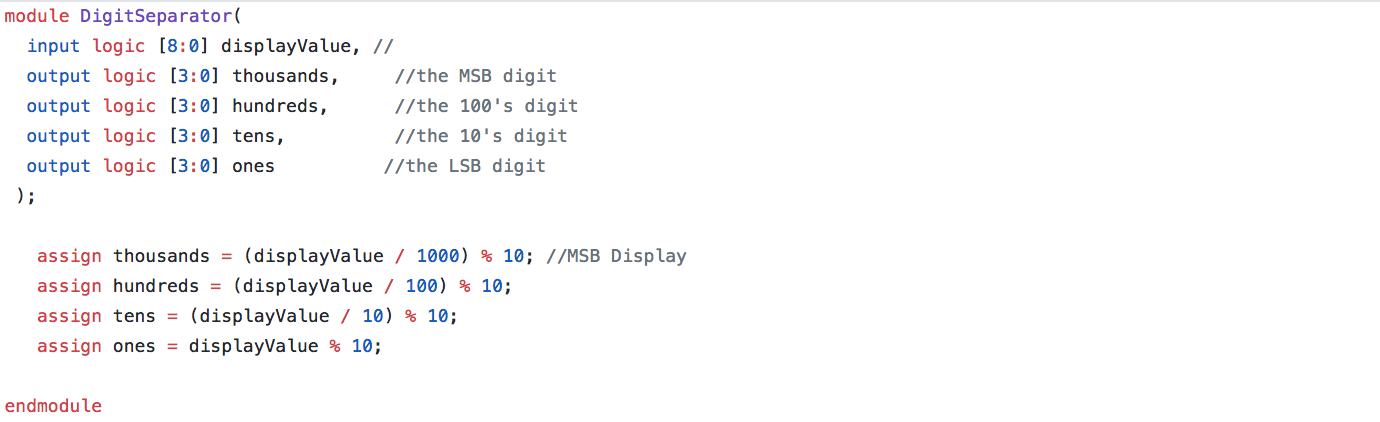
\includegraphics[width=6 in]{./Images/Archive/15-Parser.png}

\item Main Mux

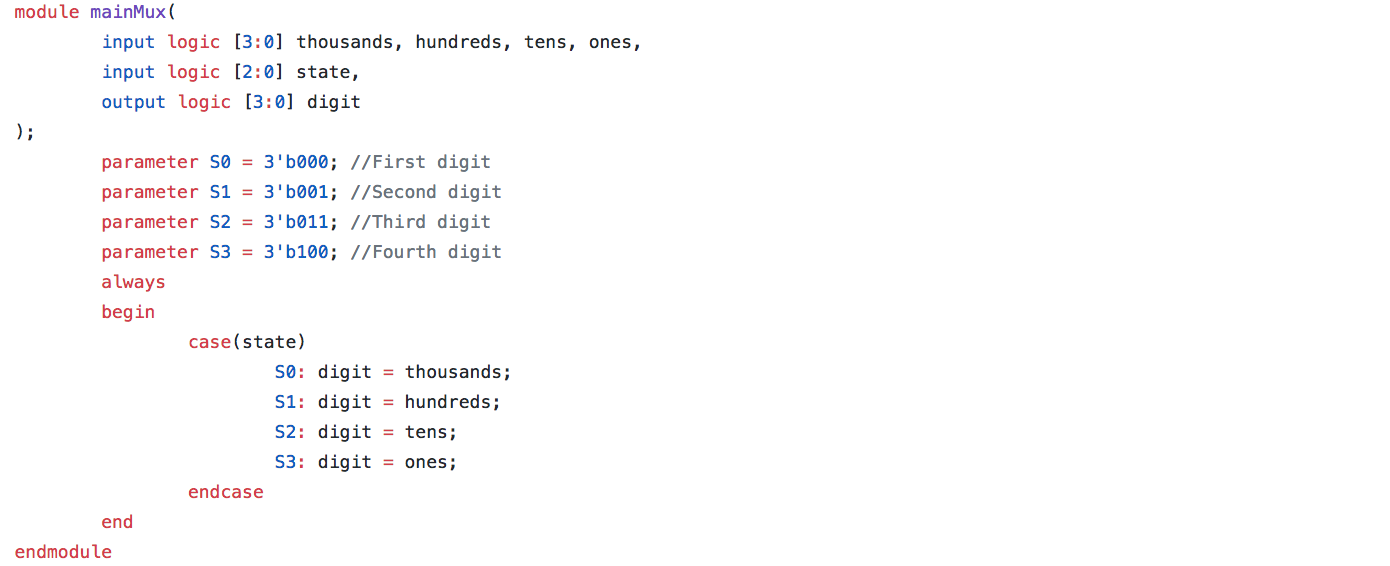
\includegraphics[width=6 in]{./Images/Archive/16-MainMux.png}

\item Segment Decoder

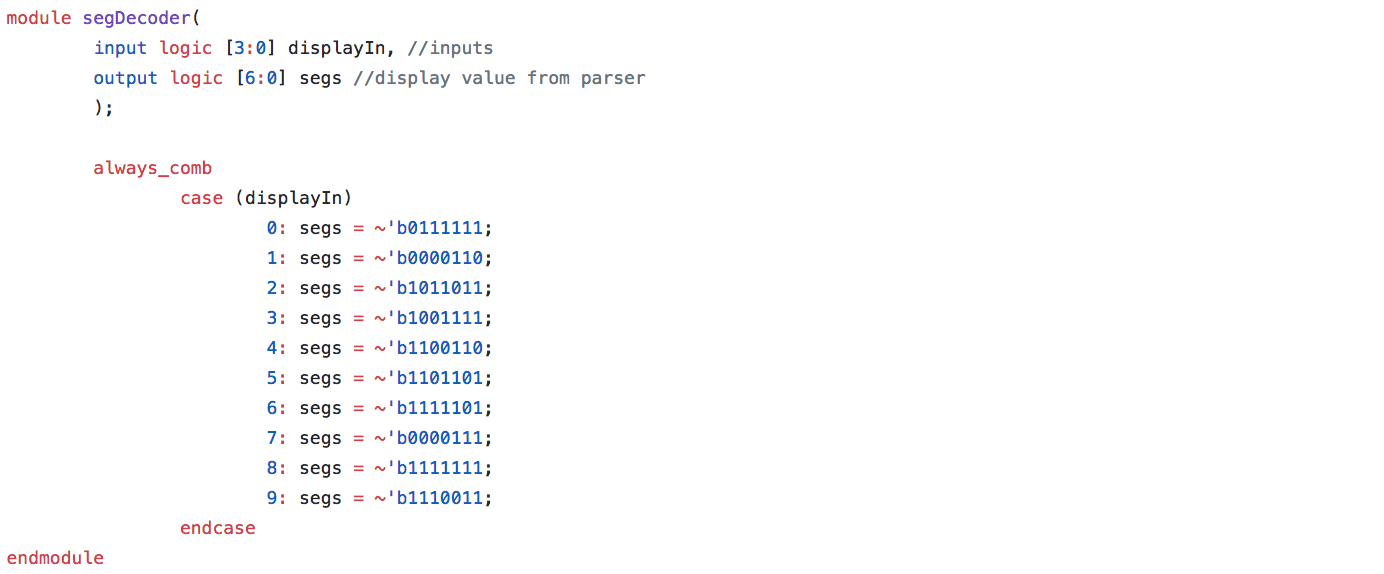
\includegraphics[width=6 in]{./Images/Archive/17-SegmentDecoder.png}

\end{enumerate}

\subsection{Testing}

\begin{enumerate}

\item Signal Generator

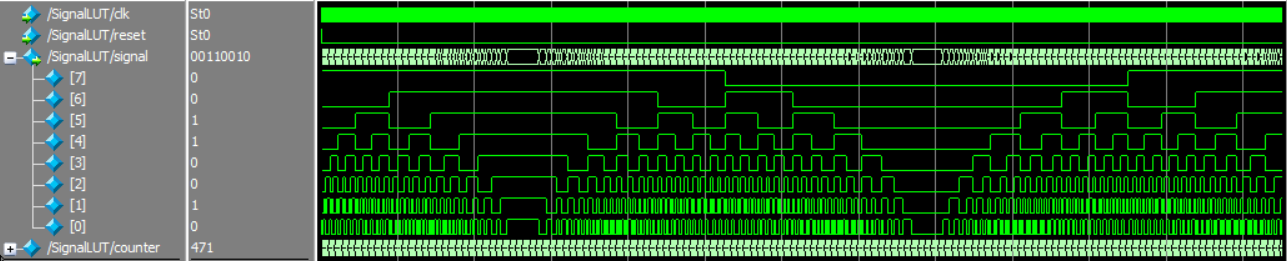
\includegraphics[width=6 in]{./Images/chasePictures/SIgnalLUTSimulation.PNG}

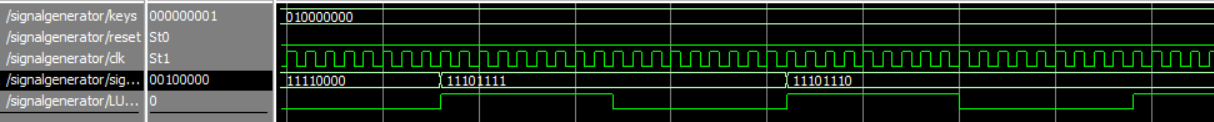
\includegraphics[width=6 in]{./Images/chasePictures/SignalGeneratorSimulation.PNG}

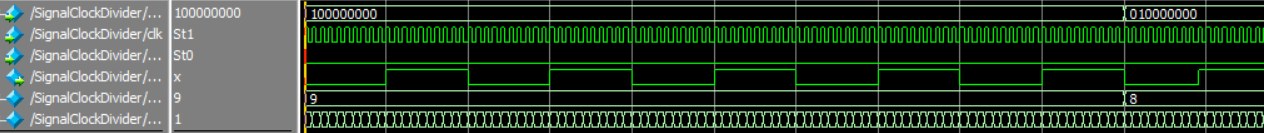
\includegraphics[width=6 in]{./Images/chasePictures/SignalClockDividerSimulation.PNG}

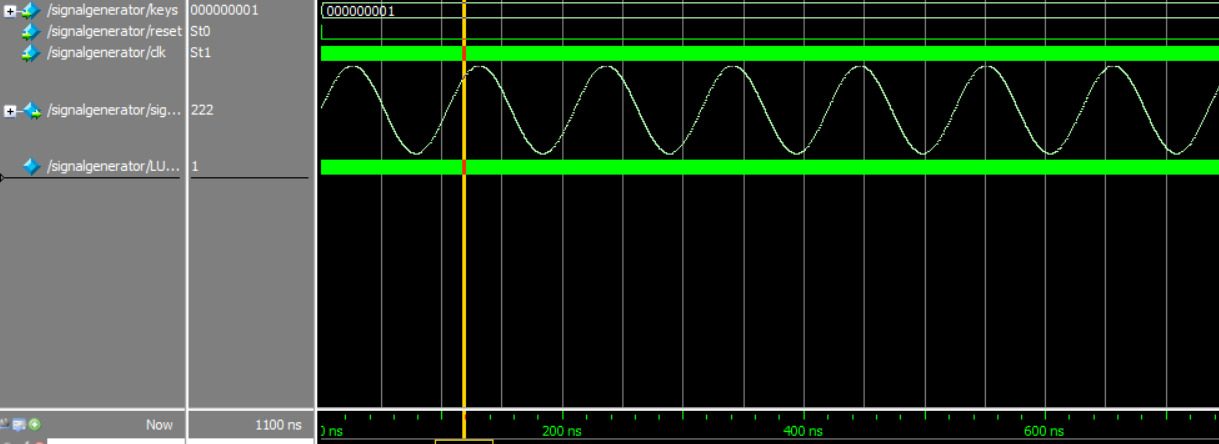
\includegraphics[width=6 in]{./Images/chasePictures/SignalGeneratorSimulationSine.PNG}

\item Segment Decoder

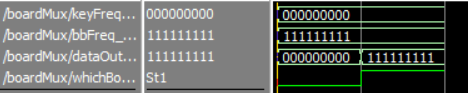
\includegraphics[width=6 in]{./Images/boardMuxSimulation.PNG}

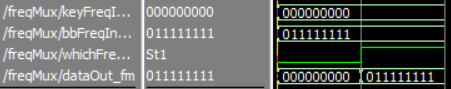
\includegraphics[width=6 in]{./Images/freqMuxSimulation.PNG}

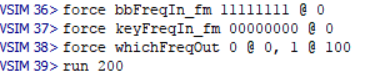
\includegraphics[width=6 in]{./Images/freqMuxSimulationDo.PNG}

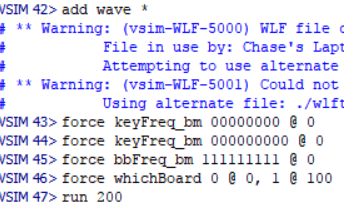
\includegraphics[width=6 in]{./Images/boardMuxSimulationDo.PNG}





\end{enumerate}



\bibliographystyle{ieeetr}
\bibliography{sample}

\end{document}